\documentclass{article}

\usepackage{array}
\usepackage{PolyTeXNancy}
% Options possibles :
%"French" ou "English" pour les titres (par défaut : French)
%"classicfont" pour revenir à la police classique LaTeX avec serif (par défaut : rien)
%"Blue", "Pink", "Green", "Orange", "Purple", "Red" ou "Grey" pour changer le thème de couleur  (par défaut : Blue)
\usepackage{multicol}
\usepackage{pdfpages}


%\usetikzlibrary{positioning,shapes,calc}

\author{Juliette Bluem}
\title{Keolis Grand Nancy}
\date{\today}

\begin{document}

% You can either have a front page with all logos using \maketitlepage
% Or simply the title before the table of content using \notitlepage
% Or both

\maketitlepage
\notitlepage

\tableofcontents

%%%%%%%%%%%%%%%%%%%%%%%%%%%%%%%%%%%%%%%%%%%%%%%%%%%%%%%%%%%%%%%%%%%%%%%%%%%%%%%%%%
\pagebreak
%---------------------------------------------------------------------------------
\section{Introduction}
Étudiante alternante, je suis en troisième année à Polytech-Nancy (= 
première année de cycle ingénieur) dans laquelle je prépare un diplôme 
d’ingénieur généraliste avec une spécialité Internet Industriel. Cette 
formation me permet de suivre principalement des cours d'informatique, 
d'automatique, de robotique, de réseaux et d'anglais. \\
En parallèle de ces cours, pour ma formation, je travaille au sein de 
l'entreprise Keolis Grand-Nancy. J'y occupe un poste d'Assistante 
Administrateur des Systèmes d'information en alternance.\\
Keolis Grand Nancy est une entreprise des transports publics, ils 
s'occupent du réseau Stan depuis 2019. En contrat depuis septembre 2020 
j'y ai travaillé deux fois quatre semaines, (que nous allons appeler périodes) 
une de mi-octobre à mi-novembre, et une de mi-décembre à mi-janvier.\\
Je vais, dans un premier temps vous présenter l'entreprise. Puis mes 
projets et misions lors de ces deux périodes.

\pagebreak
\section{Présentation de l'entreprise}

    \subsection{Global}
        \begin{figure}[!h]
            \centering
            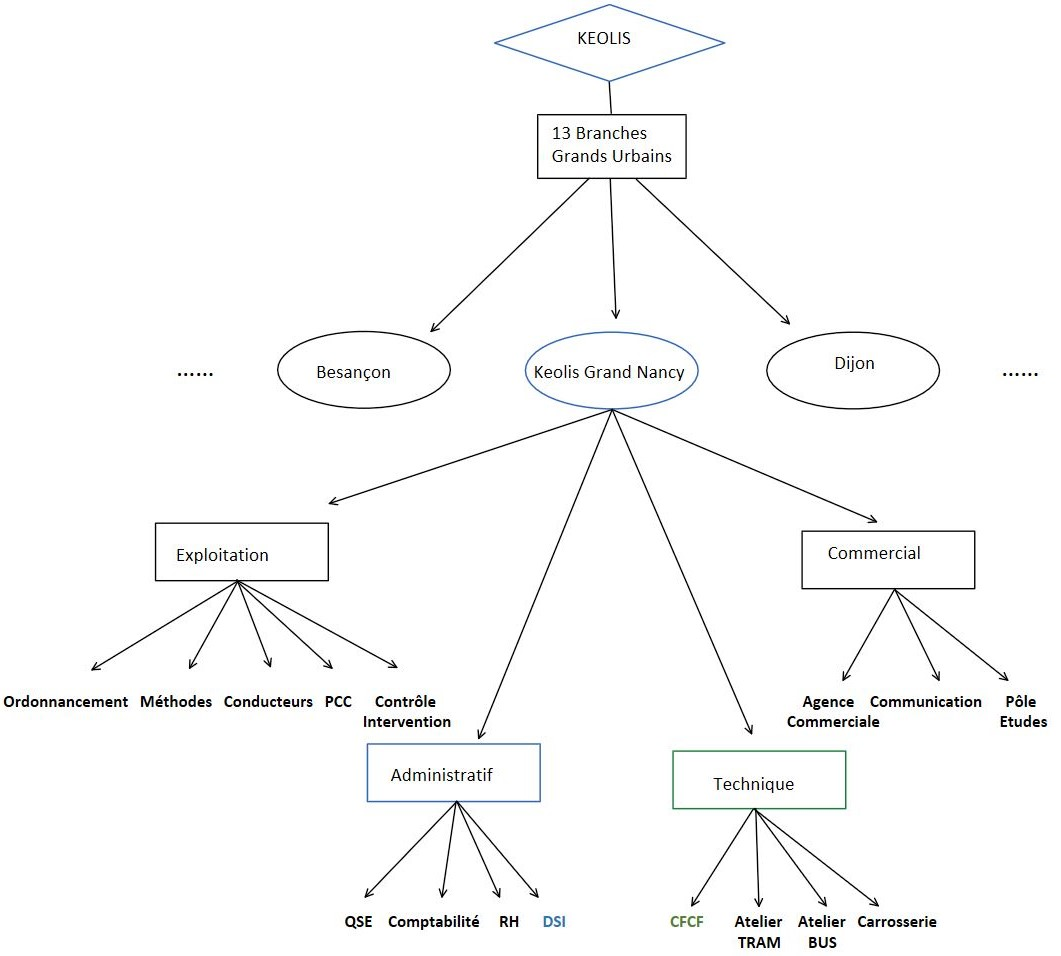
\includegraphics[scale = 0.75]{Images/Schemas_KEOLIS.JPG}
            \caption{Schémas général de mon service}
        \end{figure}

    \subsection{Le groupe Keolis}
        Le groupe Keolis, dirigé par Marie-Ange Debon, est l'un des acteurs majeurs du transport public de 
        voyageurs. Ils proposent des déplacements en métro, en tramway, en 
        train, en bus, en car ou à vélo. Ce n'est pas tout, Keolis a mis en 
        place plusieurs services d'autopartage, de transport pour personnes 
        à mobilité réduite, de stationnement ou encore de covoiturage. Keolis
        exploite également des réseaux de funiculaires, de trolleybus, de 
        navettes maritime ainsi que des services aéroportuaires. Leurs réseaux peuvent 
        être urbains, interurbains ou même périurbains.\\
        Keolis c'est aussi un chiffre d'affaire de 6.5 milliards d'euros en 2019,
        près de 70 000 collaborateurs en 2019 (dont la moitié en France), et plus 
        de 22 000 bus et cars dans le monde !\\
        L'entreprise est une filiale de la
        SNCF (70 \%). Son slogan est "More ways, more life" - que l'on peut traduire
        par "Plus de mobilité, plus de vie".

    \subsection{Keolis Grand Nancy}
        Depuis le 1er janvier 2019, KGN (Keolis Grand Nancy) gère le réseau de
        transport de la métropole du Grand-Nancy Stan par le biais d'une DSP (Délégation de service public). Xavier Lemarier en est 
        le directeur général.\\
        Le réseau Stan comprend plus de 200 véhicules dont 25 tramways, 5
        navettes électriques, 32 bus articulés au gaz naturel, 85 bus standards
        au gaz naturel, 13 minibus et 40 bus à haut niveau de service au gaz
        naturel. \\
        Stan, c'est aussi 13 lignes urbaines (dont 4 adaptées à une plus forte demande), 
        1 ligne circulaire, 4 lignes de proximité, 2 lignes citadines, 3 services de 
        transport à la demande en journée, un service de transport à la demande le dimanche, 
        un service pour rentrer de soirées, un service de nuit, un service tôt 
        le matin, 11 parkings relais et 10 parcs à vélos sécurisés et couverts.\\
        KGN est divisé en trois lieux majeurs. 
        \begin{itemize}
            \item L'agence commerciale\\ 
            Dans le hall République de la gare de Nancy, c'est avec eux que les 
            usagers échangent le plus.
            \item Le poste de commande et de contrôle\\
            Situé près de l'arrêt Mon Désert, ils ont une vision constante sur 
            tout le réseau. C'est par eux que passent les conducteurs quand ils 
            ont un problème. 
            \item Le dépôt\\
            C'est ici que reviennent les véhicules le soir. C'est également 
            ici que l'on trouve les bâtiments techniques(pour de la maintenance 
            préventive ou curative), d'exploitation (pour l'attribution 
            ligne/conducteur/véhicule) et administratif.
        \end{itemize}
        \bigbreak
        Le service de Direction des Systèmes d'information se trouve au dépôt, 
        dans le bâtiment administratif. C'est ici que travaillent mon tuteur, Olivier 
        Henriot et Sylvie Cartier, à plein temps. Théo Battin, de 
        la société OCI est également présent une fois par semaine pour 
        aider et je suis la dernière arrivée.\\
        Dans ce service, plus personne ne télétravaille. 
\pagebreak
\section{Présentation des projets et missions}

    \subsection{Période n°1}
        Je n'ai pas commencé mon expérience en entreprise dans mon service de 
        rattachement. En effet, mon tuteur entreprise, Olivier Henriot a jugé 
        intéressant, dans un premier temps, de me faire découvrir les 
        technologies utilisées par le réseau Stan. Quoi de mieux pour cela que 
        d'intégrer le service courant faible courant fort (CFCF) ? C'est donc 
        dans ce service de maintenance et d'intervention que j'ai passé mes 
        quatre premières semaines au sein de KGN.
        \subsubsection{Taches effectuées au Service CFCF}
        J'étais contente car même si je n'avais pas les compétences requises dans
        ce service, on m'a confié des tâches variées. Ce qui m'a permis de monter 
        en compétences. J'ai également pu assister les techniciens
        ce qui fu très instructif. 
        \begin{itemize}
            \item Maintenance de valideurs\\
            Les valideurs nous permettent de valider les titres de transport, c'est 
            grâce à ce matériel que nous connaissons le nombre de voyageurs. Ces 
            valideurs gèrent beaucoup de titres différents et sont souvent sujet aux 
            dégradations.\\
            Nous les démontons, retirons la poussière, changeons les pièces abimées ou en panne, 
            remontons et lavons l'extérieur. [voir \ref{Valideurs}] \\
            J'ai pu comprendre comment fonctionnait ce système que je côtoyais tous
            les jours.
            \item Test bornes wifi du dépôt\\
            Il faut savoir que tous les soirs, les bus rentrant au dépôt 
            déchargent leurs données billettiques du jour via des bornes wifi 
            réparties dans tous le dépôt. Le matin, lors de la prise de 
            services, les bus se chargent avec des données multimédia (publicité 
            de la semaine) actualisées grâce à d'autres bornes similaires. Nous 
            avons observé un problème de canal sur ces bornes (il y avait des 
            chevauchements). Nous avons donc tout refait au propre.\\
            J'ai ainsi pu mettre en pratique mes cours de protocole internet, matière
            que je découvrais en septembre. 
            \item Observation d'une intervention en sous-station\\
            Lors de ma première semaine dans le service, il fallait faire une vérification
            du bon fonctionnement des batteries au sein des sous-stations. J'ai donc pu en 
            découvrir une [voir \ref{SousStation}]. Les sous-stations alimentent le tramway. \\
            Cette demi-journée m'a permis d'avoir un rappel d'électricité sur l'intérêt 
            des onduleurs pour les batteries, mais aussi d'élargir ma culture générale
            sur la très haute tension.
            \item Dépannage d'un bus avec une panne multimédia en service\\
            Lors de sa course, le chauffeur a remarqué que ses écrans multimédia 
            étaient hors service. Nous sommes donc intervenus sur le terrain. Nous 
            avons retrouvé le bus à son terminus. Nous disposions de 10min pour 
            résoudre le problème. Il s'est avéré que c'était simplement des fils 
            débranchés. Le chauffeur a donc pu reprendre son service normalement. \\
            Ce fût une expérience intense car nous n'avions qu'un cours laps de temps pour 
            trouver et résoudre le problème, ce qui est très formateur.
            \item Mesure de hauteur de ligne\\
            \`A l'aide d'une perche isolante, nous sommes allés au carrefour 
            devant le pont Kennedy pour vérifier la hauteur de la ligne 
            électrique (nous avons pris plusieurs points de mesure et dû faire 
            face à la pluie et la circulation). Mon collègue en a profité pour
            m'expliquer l'installation électrique d'alimentation du tram. \\
            Cette demi-journée m'a principalement permis de renforcer les liens avec 
            mon collègue car nous étions responsables de la sécurité de l'autre (et nous
            étions en plein milieu d'un carrefour). Mais également d'élargir ma culture 
            générale sur la ligne aérienne.
            \item Intervention diverses sur le réseau (DAT, BIV, valideurs à quai...)\\
            Tous les jours, des DAT (distributeurs automatiques de titres), des BIV 
            (bornes information voyageurs) et des valideurs à quai tombent en 
            pannes ou sont détériorés. Il faut donc intervenir. \\
            J'ai pu développer mes compétences techniques, et surtout comprendre comment 
            fonctionnaient les différents systèmes. C'était extrêmement intéressant.
            \item Changement girouette avant, arrières et latérales de bus\\
            Les girouettes sont les indicateurs de ligne et direction (exemple : 
            T4 - Houdemont). Nous en avons changé plusieurs. Les plus 
            dérangeantes étaient celles situées à l'avant du bus car il fallait 
            les faire passer par la fenêtre du conducteur ! \\
            J'étais très contente sur la première intervention de ce genre car c'était une 
            première pour les techniciens également. Et je suis fière d'avoir eu l'idée de passer la 
            girouette par la fenêtre. Cela m'a permis de prendre confiance en moi. 
            De plus, j'ai progressé en électronique grâce à ces interventions.
            \item Changement des écrans d'un bus (obsolètes) au dépôt\\
            De façon régulière, il faut mettre le matériel embarqué dans les bus à jour. C'est ce
            que nous avons fait dans un des bus. Nous avons changé ses écrans multimédia 
            [voir \ref{Ecran}]. Ce sont des dièdres qui diffusent le trajet en cours ou 
            de la publicité. \\
            Lors de ces intervention, j'ai principalement progressé en électronique. En effet,
            lors d'un changement de matériel, nous devons refaire tous les branchements, et,
            évidemment, ce ne sont jamais les mêmes connectiques ! 
            \item Réparation de caméras \\
            Grace à un outil indiquant le bon fonctionnement des caméras dans les véhicules,
            nous avons vu que l'une des caméras était hors service. Nous en avions une autre
            en stock , également HS. Les problèmes n'étant pas les mêmes, nous avons pu faire
            de deux caméras HS une fonctionnelle [voir \ref{Camera}] que nous avons pût remettre 
            dans le véhicule de départ.\\
            Je n'étais pas en mesure de le réaliser moi-même, mais après avoir observé mon collègue,
            je serais désormais capable de le refaire.
            
        \end{itemize}
        \bigbreak

        \subsubsection{Ce que j'ai appris au Service CFCF}
        Pendant ces quatre semaines au sein de ce service, j'ai 
        développé des compétences techniques. J'ai également progressé 
        dans ma démarche de résolution d'un problème. Et surtout, j'ai pu 
        découvrir toutes les technologies utilisées par le réseau Stan. \^Etre 
        directement dans un service de maintenance et d'intervention m'a permis
        de réellement comprendre le fonctionnement du matériel embarqué. J'ai 
        également pu comprendre comment travaillaient les techniciens de ce 
        service, cela va me permettre de plus facilement travailler avec eux 
        dans le futur.


    \subsection{Période n°2 - Comptage}
        Pour ma deuxième période, j'ai intégré le service de Direction des 
        Systèmes d'information.\\
        Mon tuteur m'a expliqué les différents projets en cours. Un des plus 
        importants répond à une problématique de comptage. En effet, depuis début
        décembre, le réseau Stan est gratuit les samedis et les dimanches. Or, 
        sans validation des voyageurs, nous ignorons combien de personnes ont 
        voyagé sur le réseau dans la journée. Il faut donc trouver une
        solution de comptage des voyageurs. Deux sont "présélectionnées" :
        DotPulse (pour la ligne 1) et Acorel (pour la ligne 4).

        \subsubsection{DotPulse}
        La technologie DotPulse est un boitier d'analyse de flux wifi et gsm. 
        Vous trouverez en annexes un schéma clair représentant ce fonctionnement. 
        [voir \ref{DotPulse_Technologie}] Cette technologie, en plus de répondre 
        au premier besoin permettrait de collecter davantage d'informations très utiles pour 
        l'analyse du réseau.\\
        Ce projet est encore loin d'être abouti. Pour le moment, seuls deux boitiers 
        sont en service, ils ont servi de "premier jet" pour l'installation et le positionnement
        dans les véhicules. 12 boitiers identiques seront installés en avril, ce qui permettra 
        de débuter réellement l'étude de performance. Ces 14 boitiers seront positionnés dans des tramways
        de la ligne 1 (ligne la plus influente du réseau).

        En décembre, j'ai pris connaissance de ce projet et de cette technologie. Afin 
        de mieux m'imprégner du sujet, j'ai réalisé une présentation de DotPulse 
        et du projet KGN x Kisio (société proposant DotPulse) [voir \ref{DotPulse_Presentation}]. Le but était dans 
        un premier temps d'expliquer à la métropole du Grand Nancy ce projet, et, dans un 
        second temps de m'exercer à la présentation et aux outils de gestion de projet.\\
        En effet, pour cette présentation, j'ai réalisé tout un planning qui devait 
        être clair et concis [voir \ref{DotPulse_Gantt}]. Je l'ai réalisé sur Excel à la manière d'un diagramme de Gantt.
        J'ai également dû prendre contact avec les équipes du service courant faible courant
        fort afin d'estimer le temps d'installation des boitiers. Il a ensuite fallu que je
        contacte le service technique des tramways, afin de savoir quand nous pouvions mettre 
        à l'arrêt des tramways pour installer DotPulse. Cette tâche m'a permis d'améliorer mes 
        compétences organisationnelles.

        \subsubsection{Acorel}
        La technologie d'Acorel [voir \ref{Acorel_techno}] est actuellement installée sur 
        la ligne T4 (depuis 2017). Afin de verrifier sa précision, nous devons comparer les données renvoyées 
        par la billettique déjà installée avec celles renvoyées par les cellules Acorel. \\
        Les données issues de la billettique comme celles des cellules Acorel sont exportables.
        Nous récupérons donc pour chacune d'elles un document .cvs contenant énormément d'informations.
        J'ai eu pour tâche d'extraire les informations utiles à notre étude. Puis, je les
        ai organisées (sous forme d'un tableau lisible regroupant pour chaque type de données et chaque 
        jour, le nombre de montées). Ensuite, j'ai procédé à l'analyse de ce tableau. Pour cela, j'ai réalisé
        un tableau comparatif avec un code couleur simple.[voir \ref{Acorel_etudes}] Grâce à ces opérations, nous
        voyons que des bus ont des erreurs récurentes, nous les avons évidement signalées à la 
        maintenance pour qu'ils agissent sur les cellules.\\
        Bien évidemment tout n'a pas fonctionné du premier coup. Initialement, nous récupérions de 
        la part d'Acorel des données traitées, ce qui faussait totalement nos résultats. Nous 
        leur avons demandé d'avoir les données brutes. Cela a rendu notre étude beaucoup plus 
        concluante.


    \subsection{Période n°2 - Autres projets}

        \subsubsection{Compta \& DAT}
        Nous avons également évoqué un problème de remontée d'informations. En
        effet, le service de comptabilité n'est pas en mesure de faire la différence entre
        un DAT HS et un DAT non-utilisé. Des mails sont échangés régulièrement entre le 
        SCFCF et le service comptabilité à ce sujet. Une 
        solution serait de remonter les interventions du SCFCF à la comptabilité. J'ai
        commencé ce projet fin décembre et continuerai à mon retour en février.

        \subsubsection{Inventaire}
        Nous avons dû mettre à jour l'inventaire des postes de travail du dépôt [voir \ref{Gpli_ex}]. 
        Pour cela, je devais noter plusieurs informations de connexion pour 
        chaque poste de travail actif [voir \ref{Gpli_papier}]. Cela permet de tenir à jour notre base 
        de données. Avoir réalisé cette démarche m'a permis de me familiariser 
        avec le site et les travailleurs. Ce fut un exercice compliqué car beaucoup 
        de personnes étaient en télétravail ou en vacances, mais important et 
        intéressant. Je n'ai pas pu finir cette tâche, je la poursuivrai en février.

        \subsubsection{Borne d'information dépôt}
        Nous pourrions également améliorer la communication au sein du dépôt en 
        modifiant l'affichage dans le hall d'accueil. Actuellement un 
        paperboard est disposé à l'entrée du bâtiment, il affiche diverses 
        informations sur l'entreprise. Nous pensons pouvoir moderniser cet 
        affichage en ajoutant un écran. Cela nous permettrait également 
        d'afficher des informations dynamiques telles que les horaires des 
        prochains passages de bus autour du dépôt (Polytech Nancy dispose de ce genre 
        d'affichage dans les halls des bâtiments E et F). Je vais donc me charger 
        de ce petit projet. J'ai commencé en janvier et finirai à mon retour en 
        février.

    \subsection{Ce que j'ai appris à la DSI}
        Lors de cette période à la DSI, j'ai pu tout d'abord découvrir l'équipe avec laquelle 
        je vais travailler. Ces derniers m'ont d'ailleurs rapidement mis en confiance.\\
        J'ai très rapidement pu mettre en pratique mes comptétences en gestion de projet, 
        c'est un exercice que j'apprécie particulièrement, j'en était donc ravie.\\
        Grâce notamment à l'étude Acorel, j'ai beaucoup progressé sur Excel, outil que 
        j'utilisais très bien, mais d'un point de vue bureautique et mathématique 
        uniquement.\\
        De plus, j'ai fortement consolidé mes bases, en matière de recherche. 
        En effet, face à un problème ou un exercice inconnu, j'ai du trouver des solutions
        seule avant de trouver de l'aide autour de moi. Ce genre d'exercice
        me fait rapidement progresser et permet de développer mon autonomie.

\pagebreak
\section{Bilan}
    J'ai passé deux périodes en entreprise extrêmement enrichissantes. Toutes deux bien 
    distinctes, certes, mais toutes deux très complémentaires en un sens. Comme l'avait, à 
    très juste titre, anticipé mon tuteur, mon expérience dans le service courant faible courant 
    fort m'a été très utile au service informatique. Elle m'a permis de participer activement aux 
    projets. Je me suis sentie beaucoup plus utile grâce à elle.\\
    Bien que mon tuteur ait tout mit en oeuvre pour lever mes appréhensions avant mon entrée dans l'entreprise, 
    je n'ai pas pu m'empêcher de ressentir une légère inquiétude au départ.
    C'était clairement infondé, les équipes que j'ai côtoyées ont toutes été très chaleureuses,
    compréhensives, respectueuses et à l'écoute de mes avis.\\
    D'un point de vue scolaire, je parviens à faire le lien entre certains de mes cours et ce 
    que je fais en entreprise, 
    c'est très intéressant, cela me donne un autre regard sur les cours en question. Lors de mes 
    prochaines périodes en entreprise, je sais que je vais mettre en application des cours 
    supplémentaires, comme celui sur les bases de données qui devrait faciliter la réalisation du projet 
    de lien entre le service comptabilité et le service courant faible courant fort pour les DAT par exemple.\\
    
    
\pagebreak
\section{Annexes}
    
    \subsection{Missions SCFCF}

        \subsubsection{Valideurs}
            \label{Valideurs}
            \begin{figure}[!h]
                \centering
                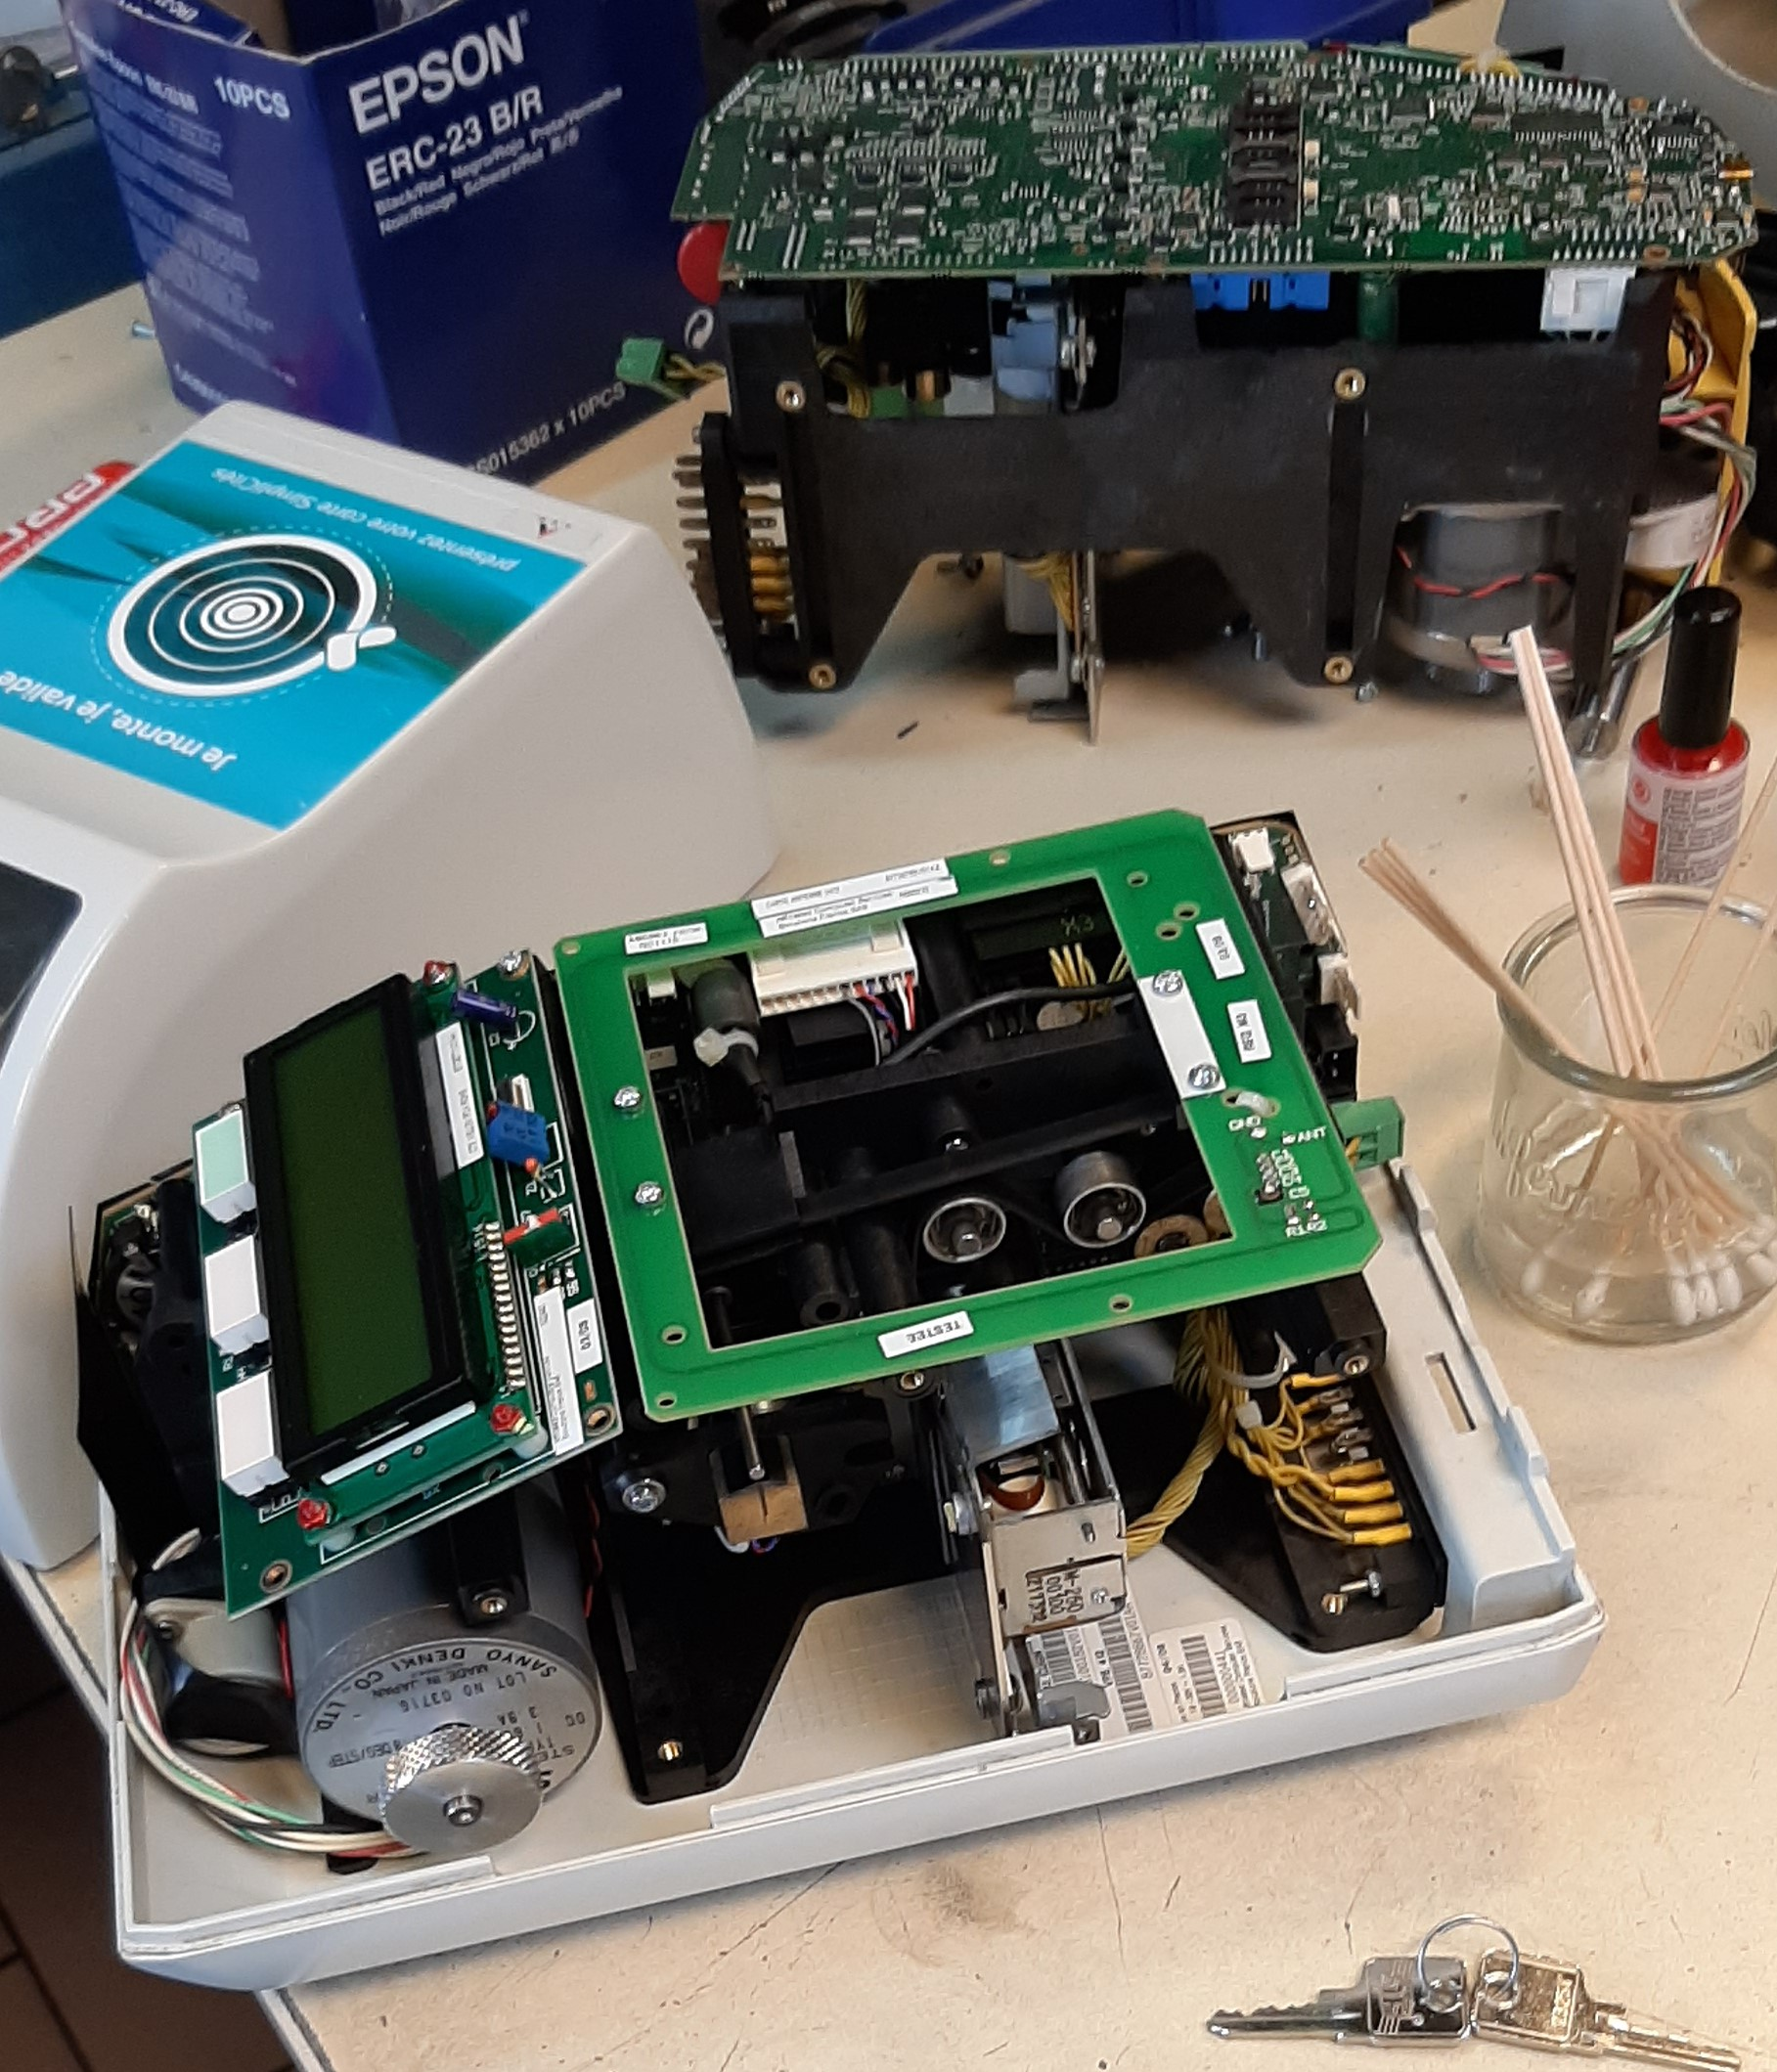
\includegraphics[scale = 0.1]{Images/valideur.jpg}
                \caption{Maintenance d'un valideur embarqué}
            \end{figure}

        \subsubsection{Sous Station}
            \label{SousStation}
            \begin{figure}[!h]
                \centering
                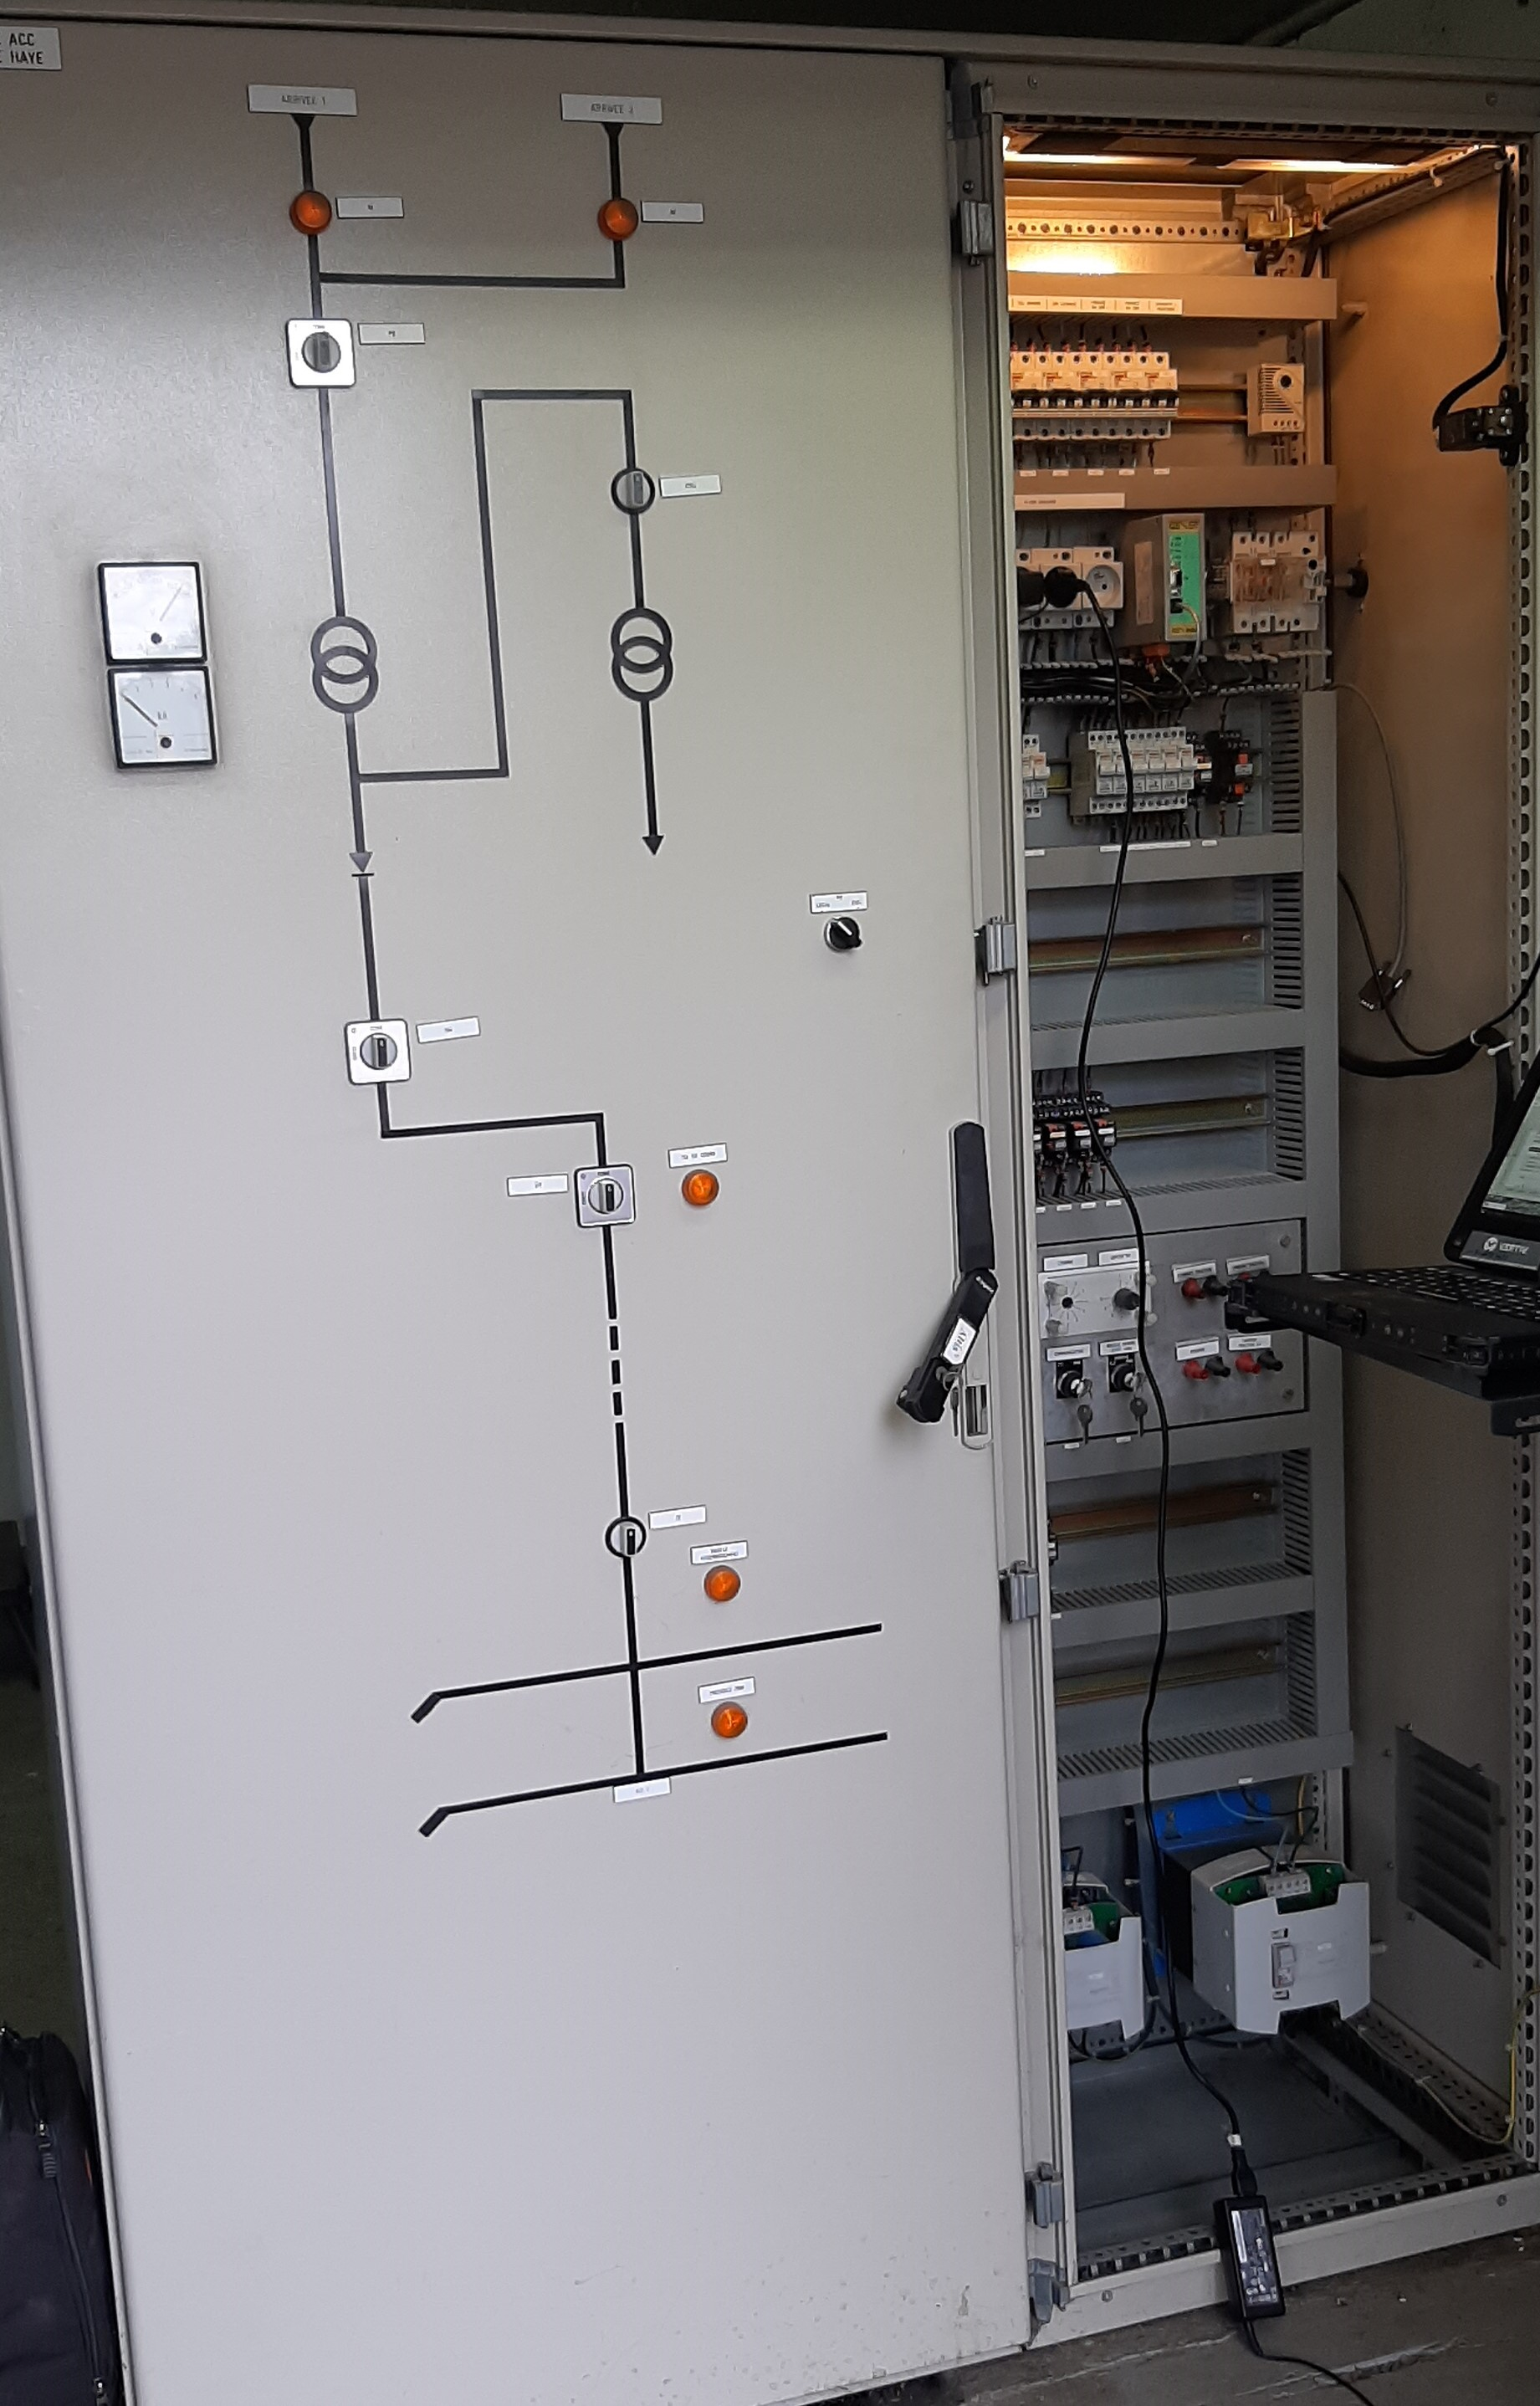
\includegraphics[scale = 0.1]{Images/sousStation1.jpg}
                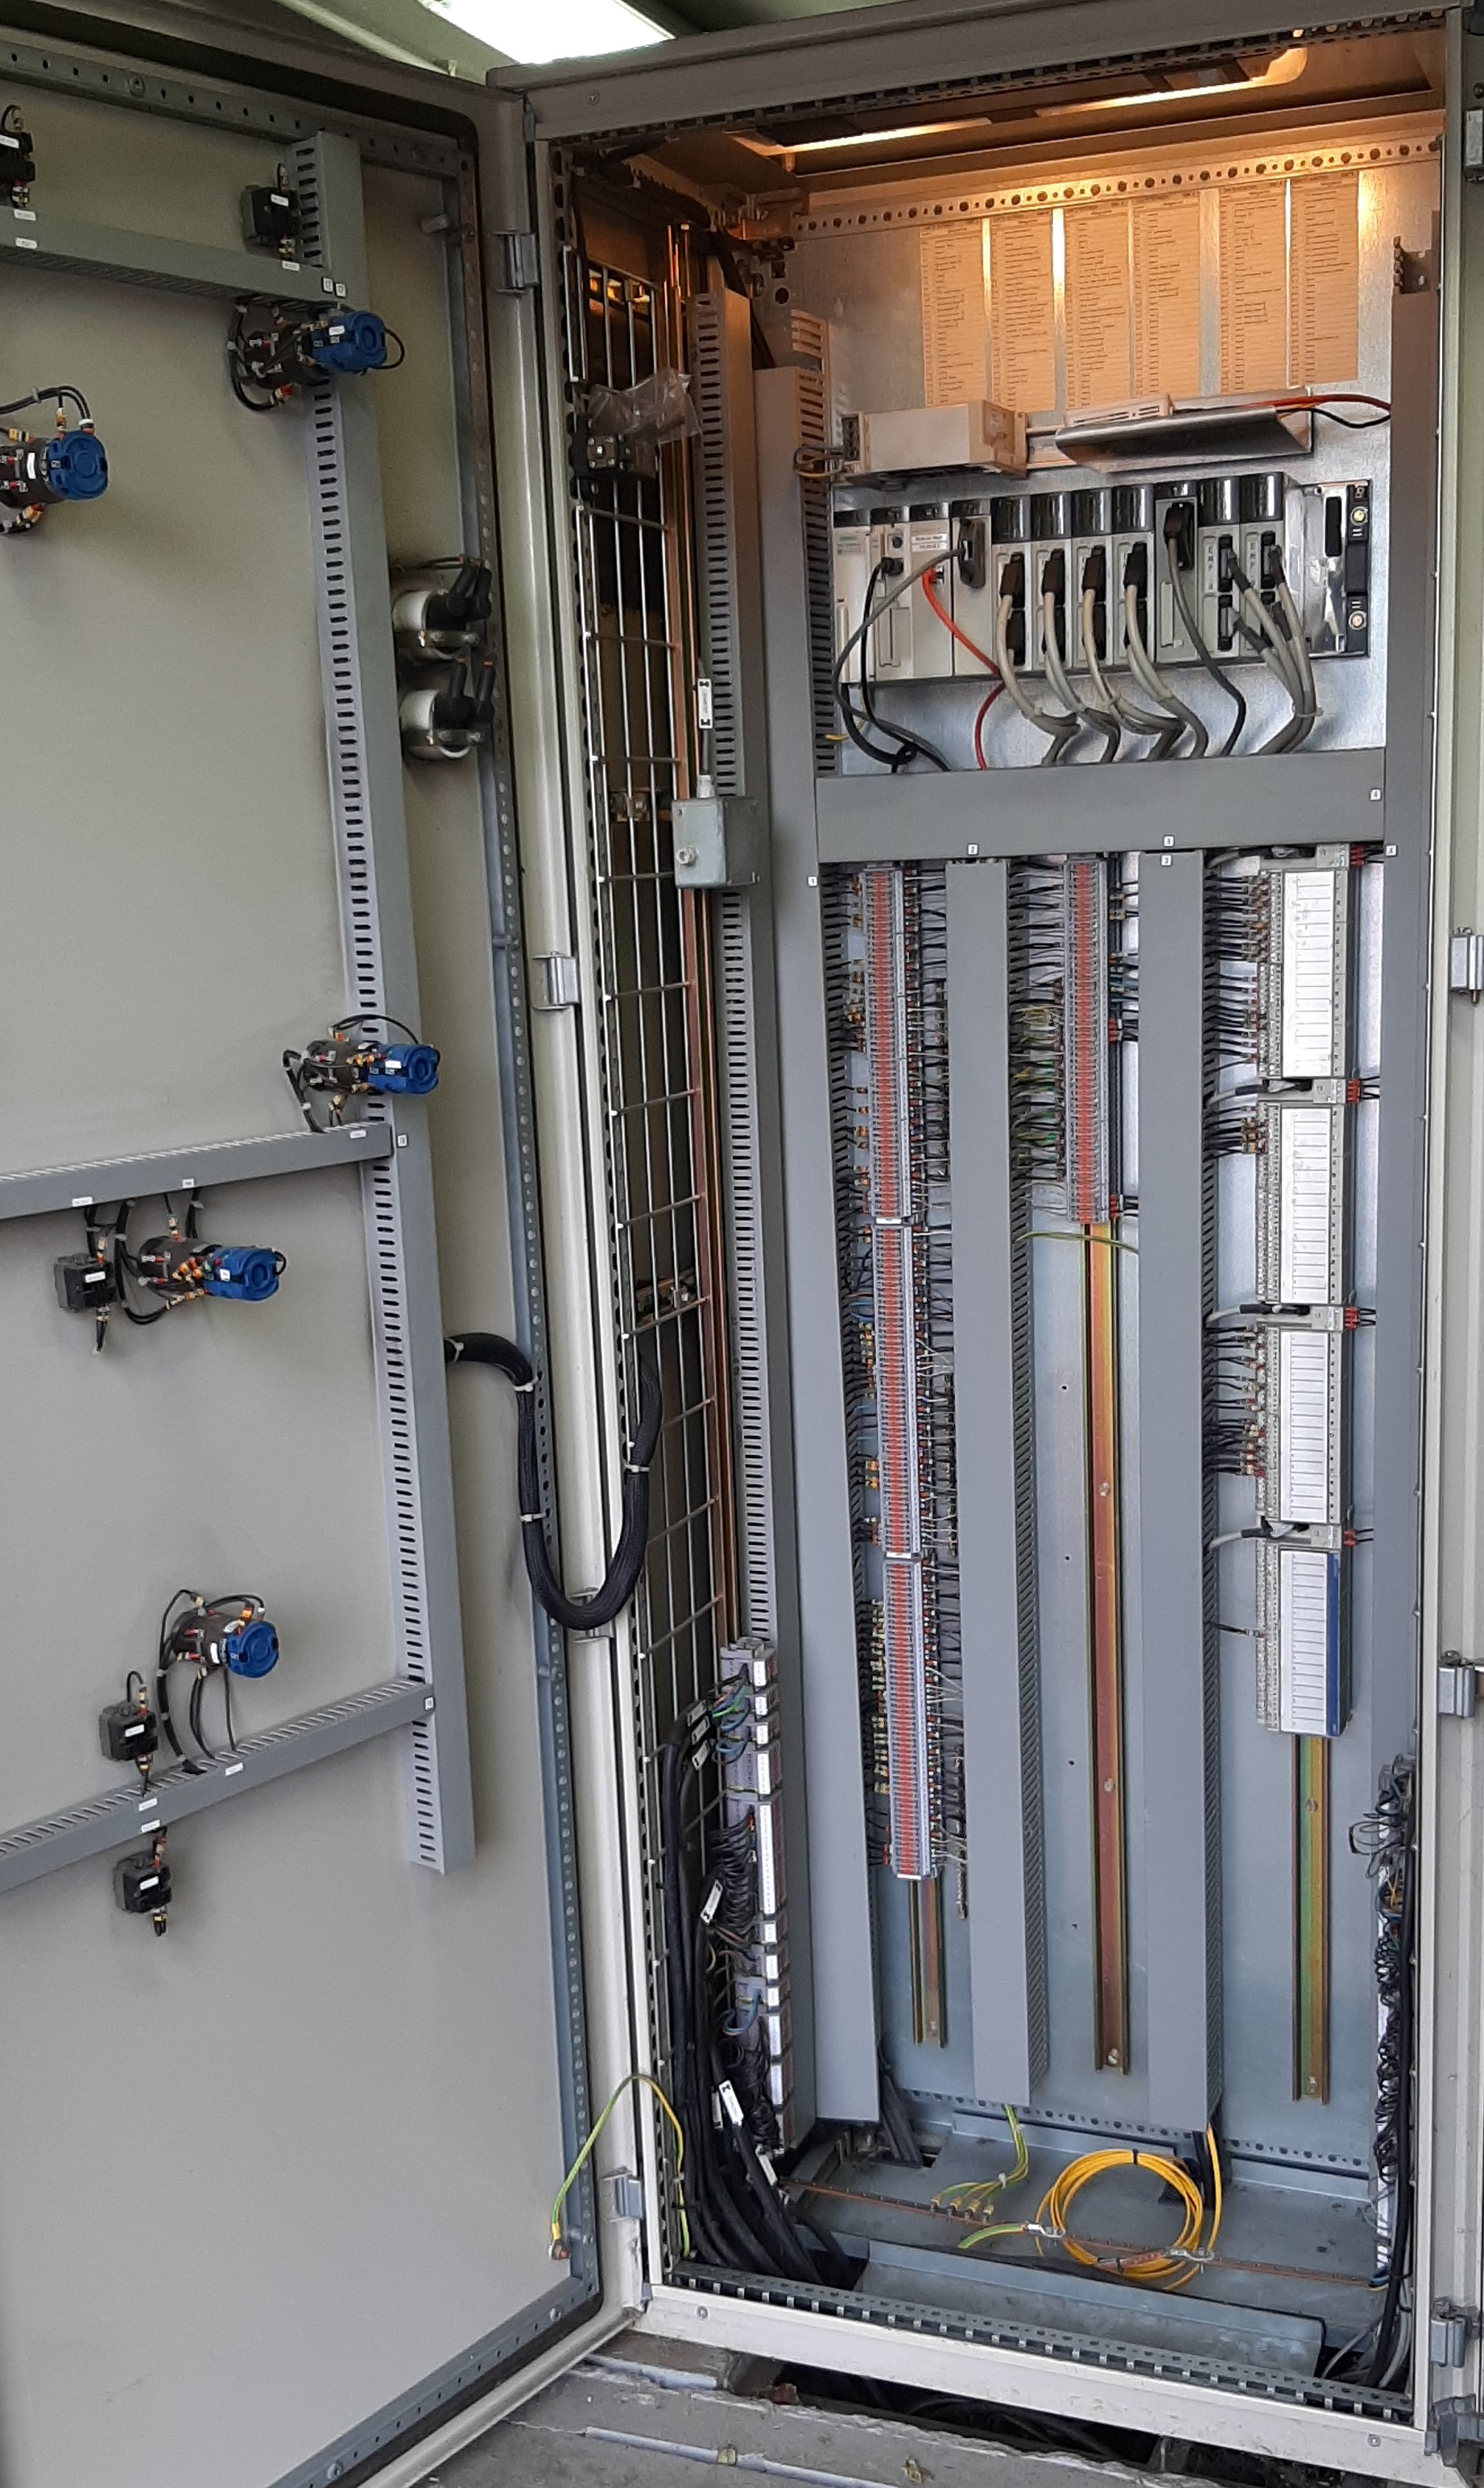
\includegraphics[scale = 0.1]{Images/sousStation2.jpg}
                \caption{Armoire en sous-station}
            \end{figure}

        \pagebreak
        \subsubsection{Changement écran}
            \label{Ecran}
            \begin{figure}[!h]
                \centering
                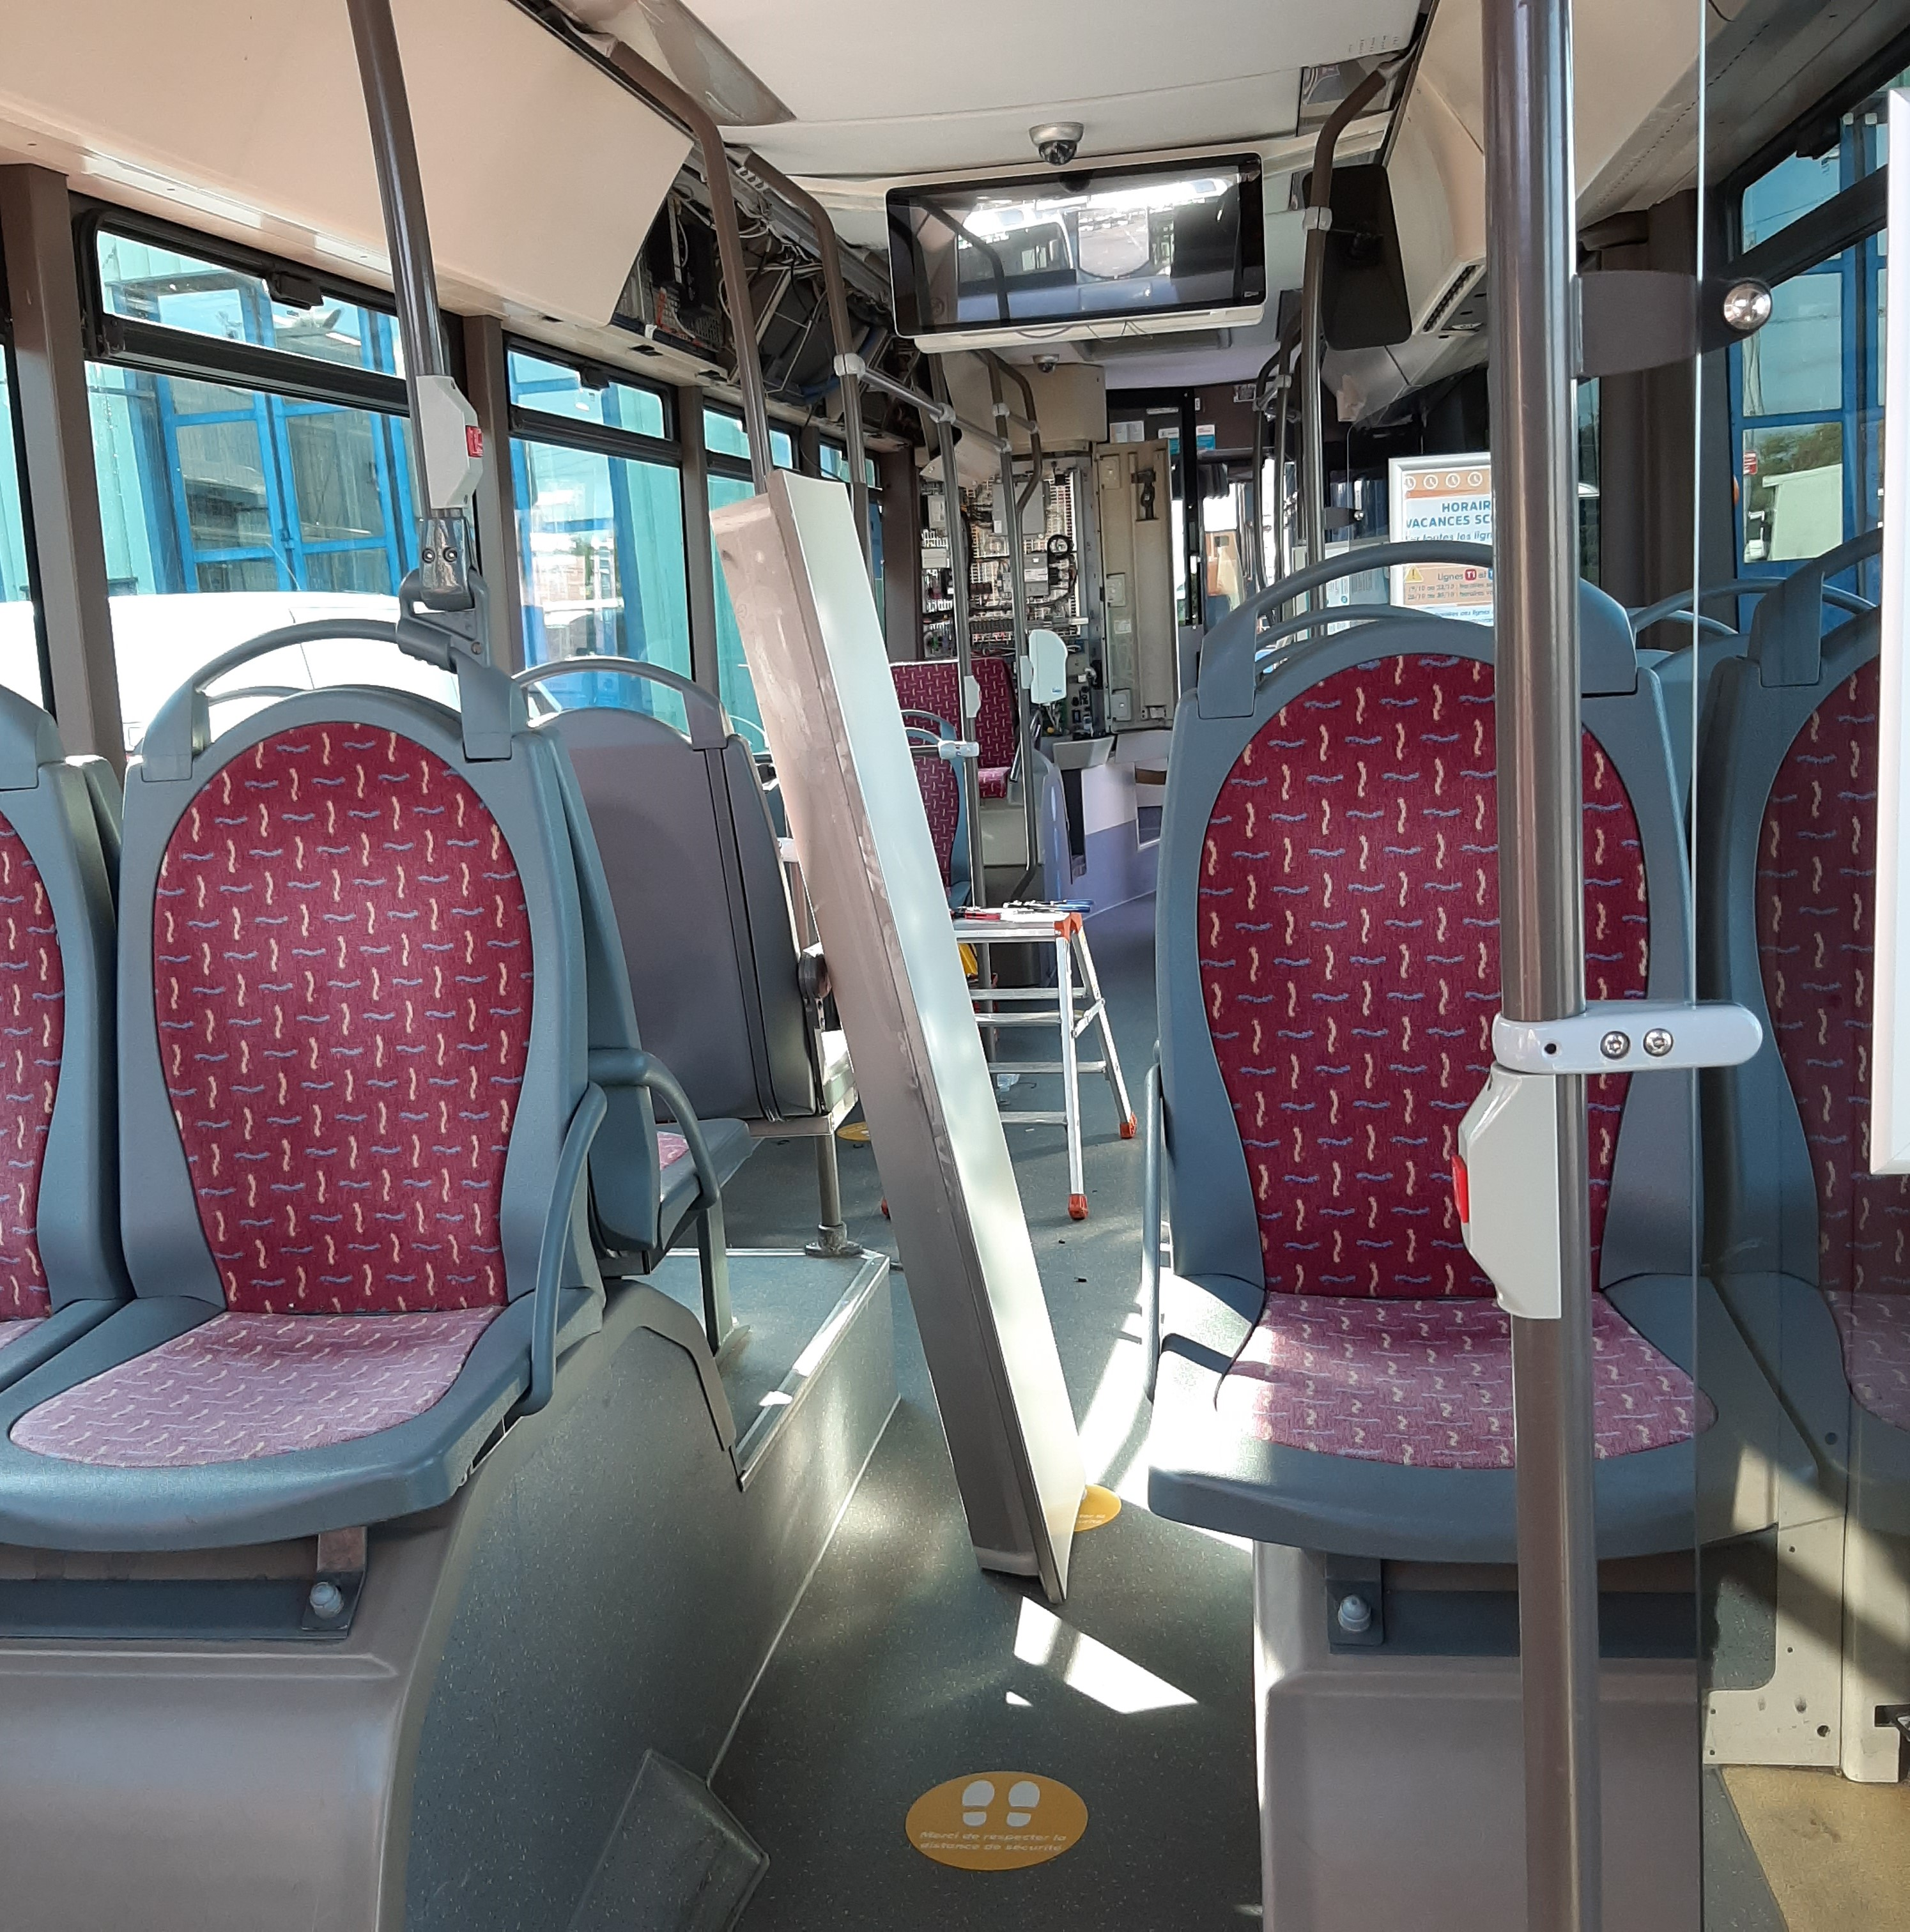
\includegraphics[scale = 0.1]{Images/multimedia.jpg}
                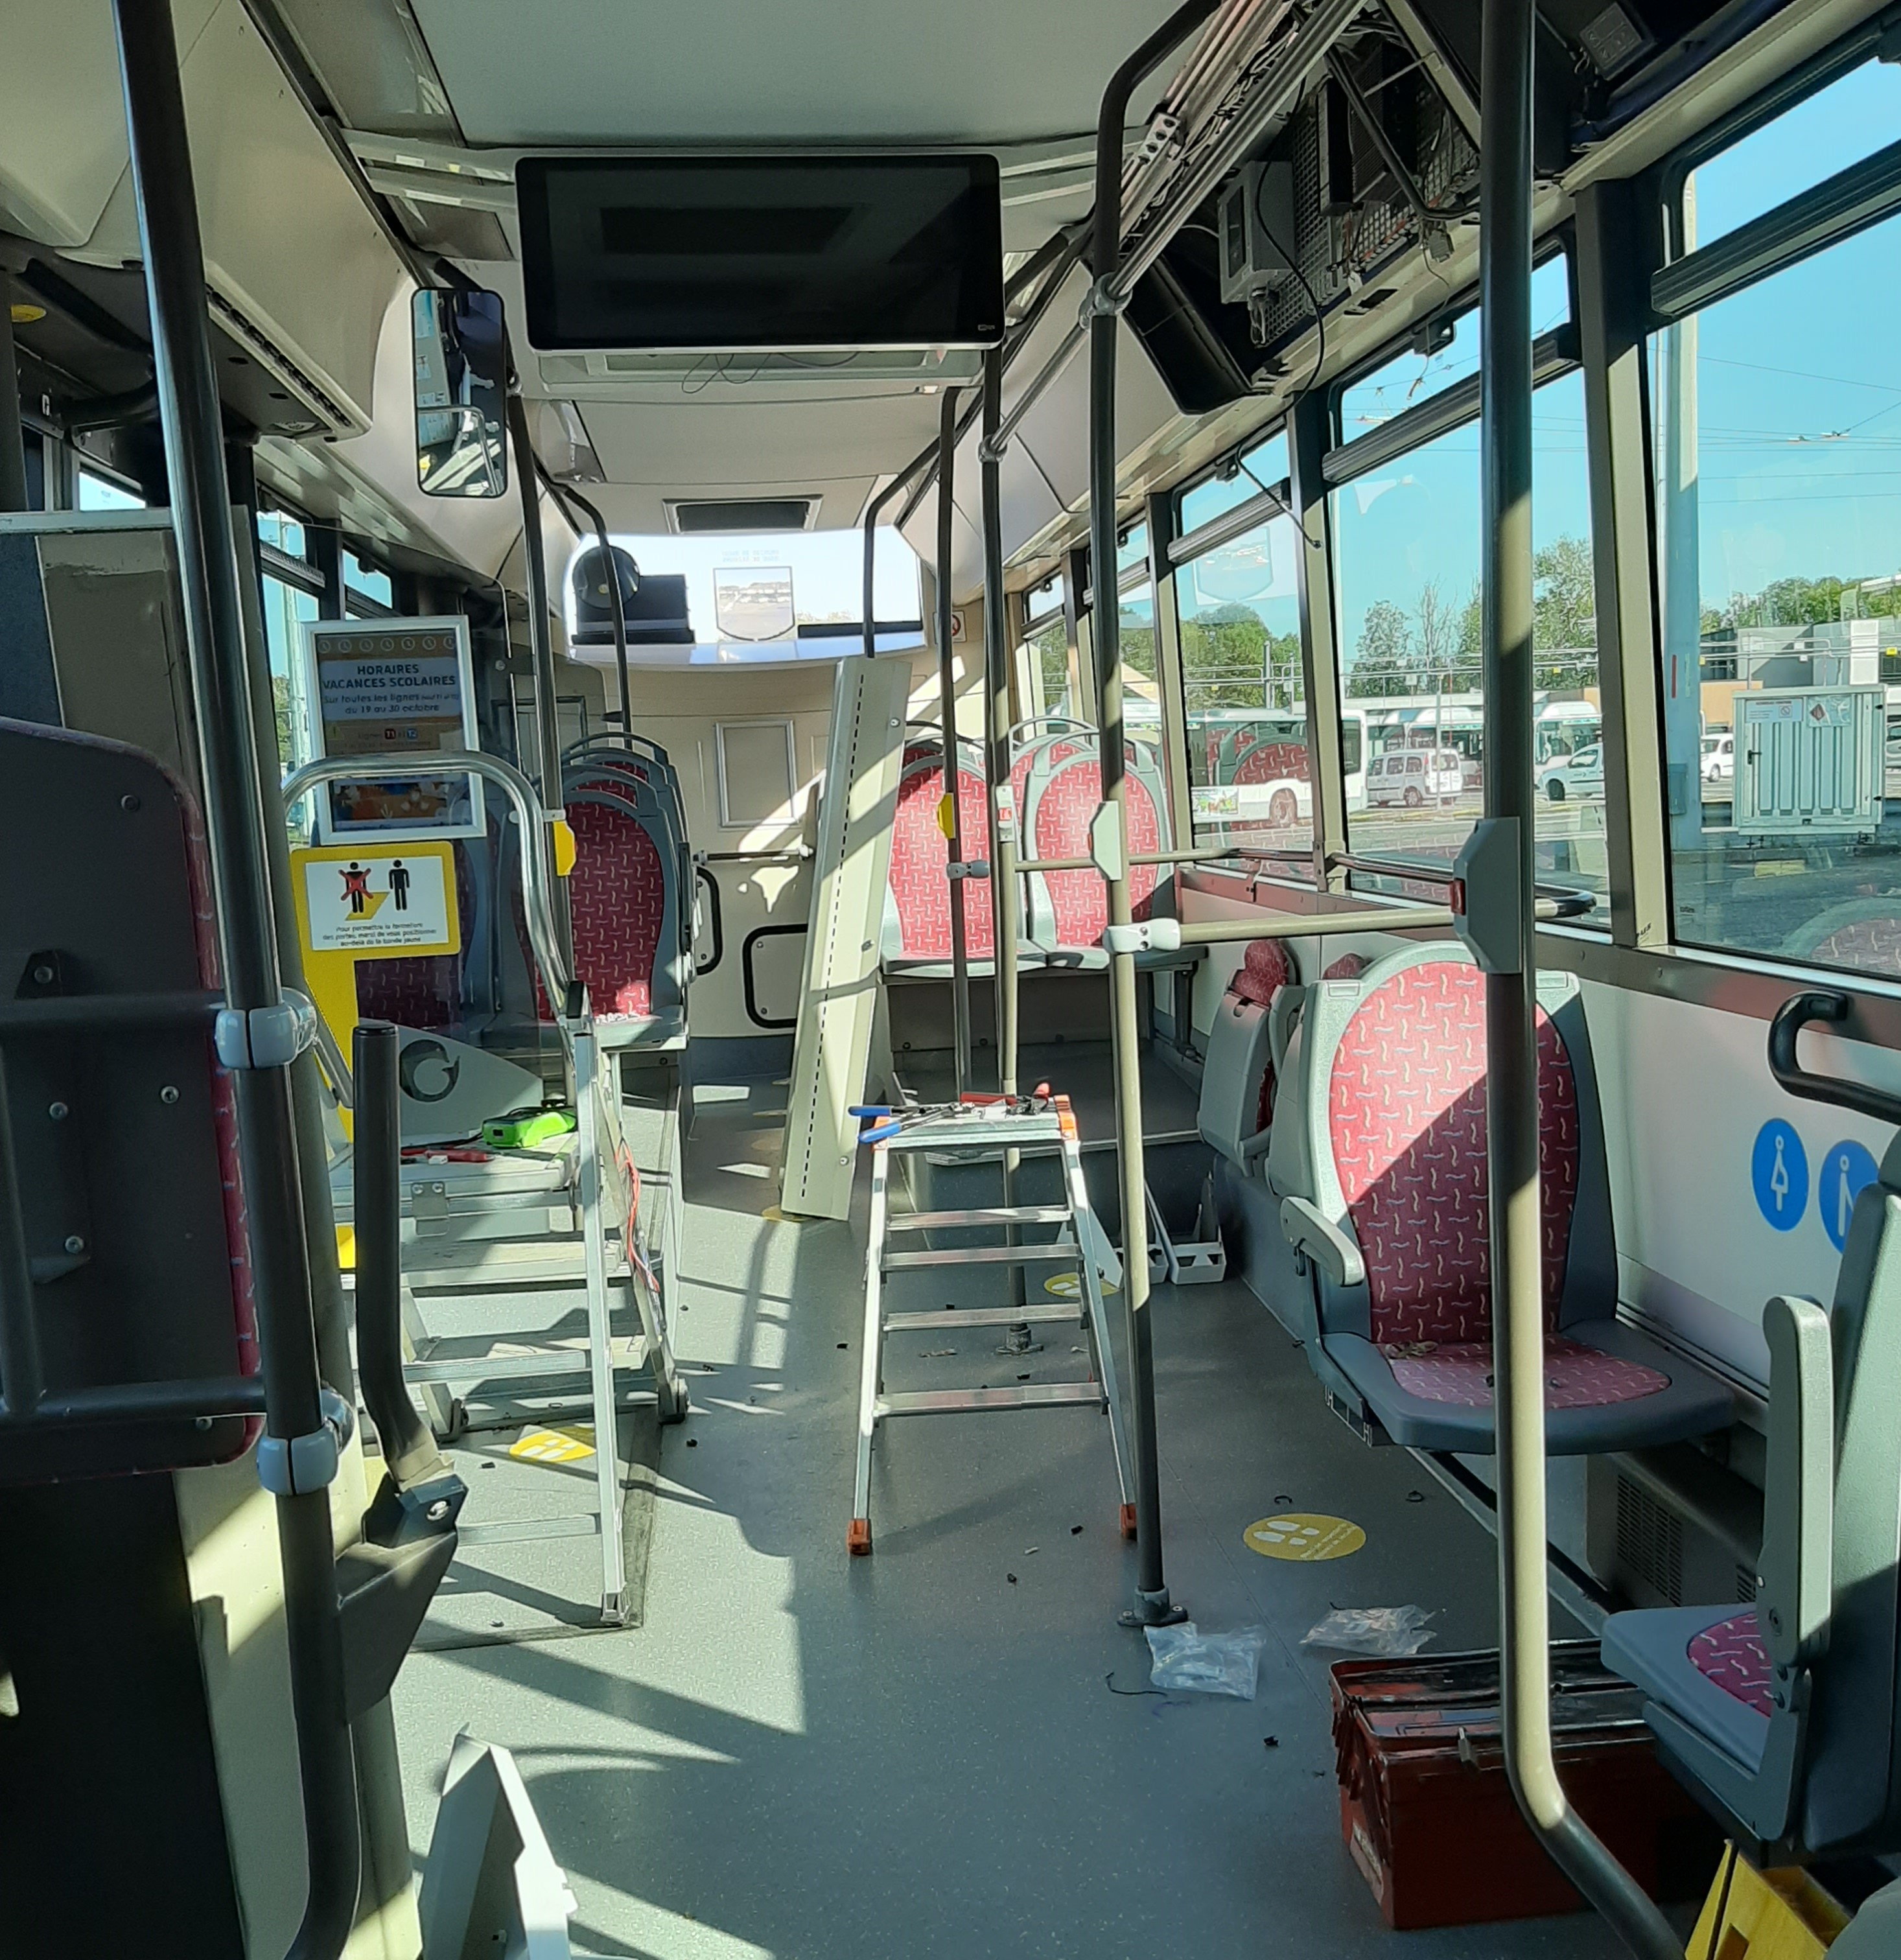
\includegraphics[scale = 0.1]{Images/multimedia2.jpg}
                \caption{Changement des dièdres multimédia}
            \end{figure}

        \subsubsection{Réparation de caméras}
            \label{Camera}
            \begin{figure}[!h]
                \centering
                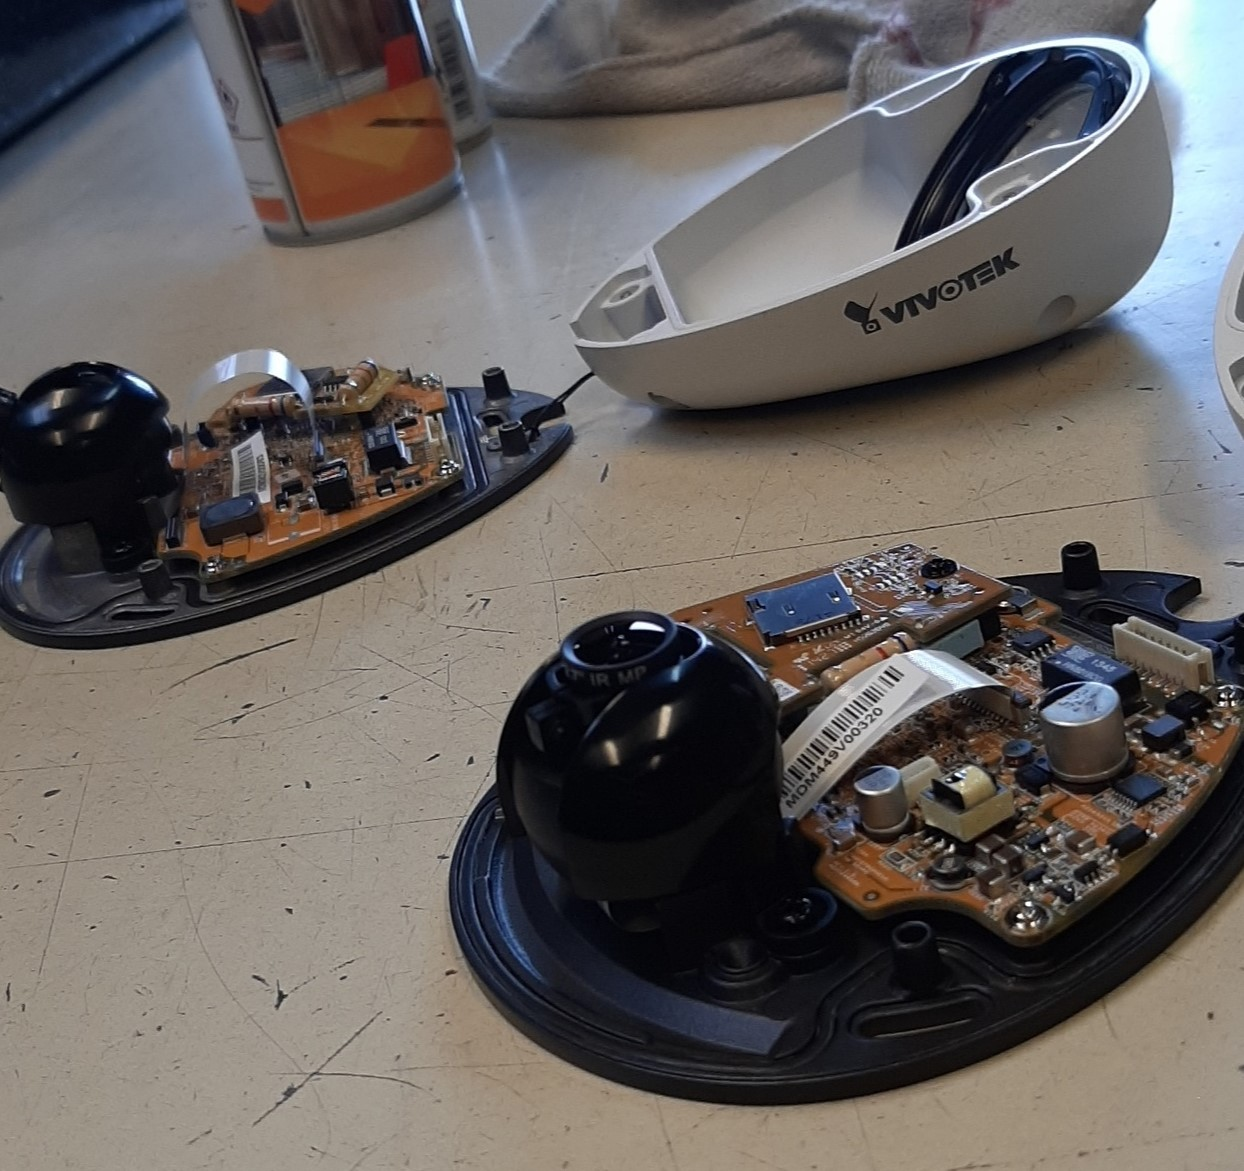
\includegraphics[scale = 0.1]{Images/camera.jpg}
                \caption{Faire une caméra fonctionnelle avec deux défectueuses}
            \end{figure}


    \pagebreak
    \subsection{DotPulse}

        \subsubsection{La technologie}

            \label{DotPulse_Technologie}
            \begin{figure}[!h]
                \centering
                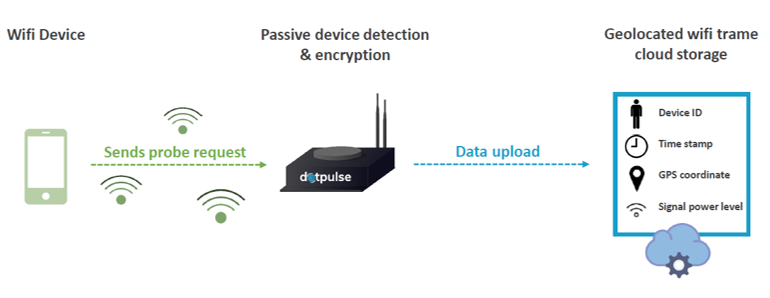
\includegraphics[scale = 0.4]{Images/principe_dotPulse.png}
                \caption{Présentation du principe de fonctionnement de DotPulse (doc Kisio)}
            \end{figure}

        \subsubsection{Présentation}

            \label{DotPulse_Presentation}
            \begin{figure}[!h]
                \centering
                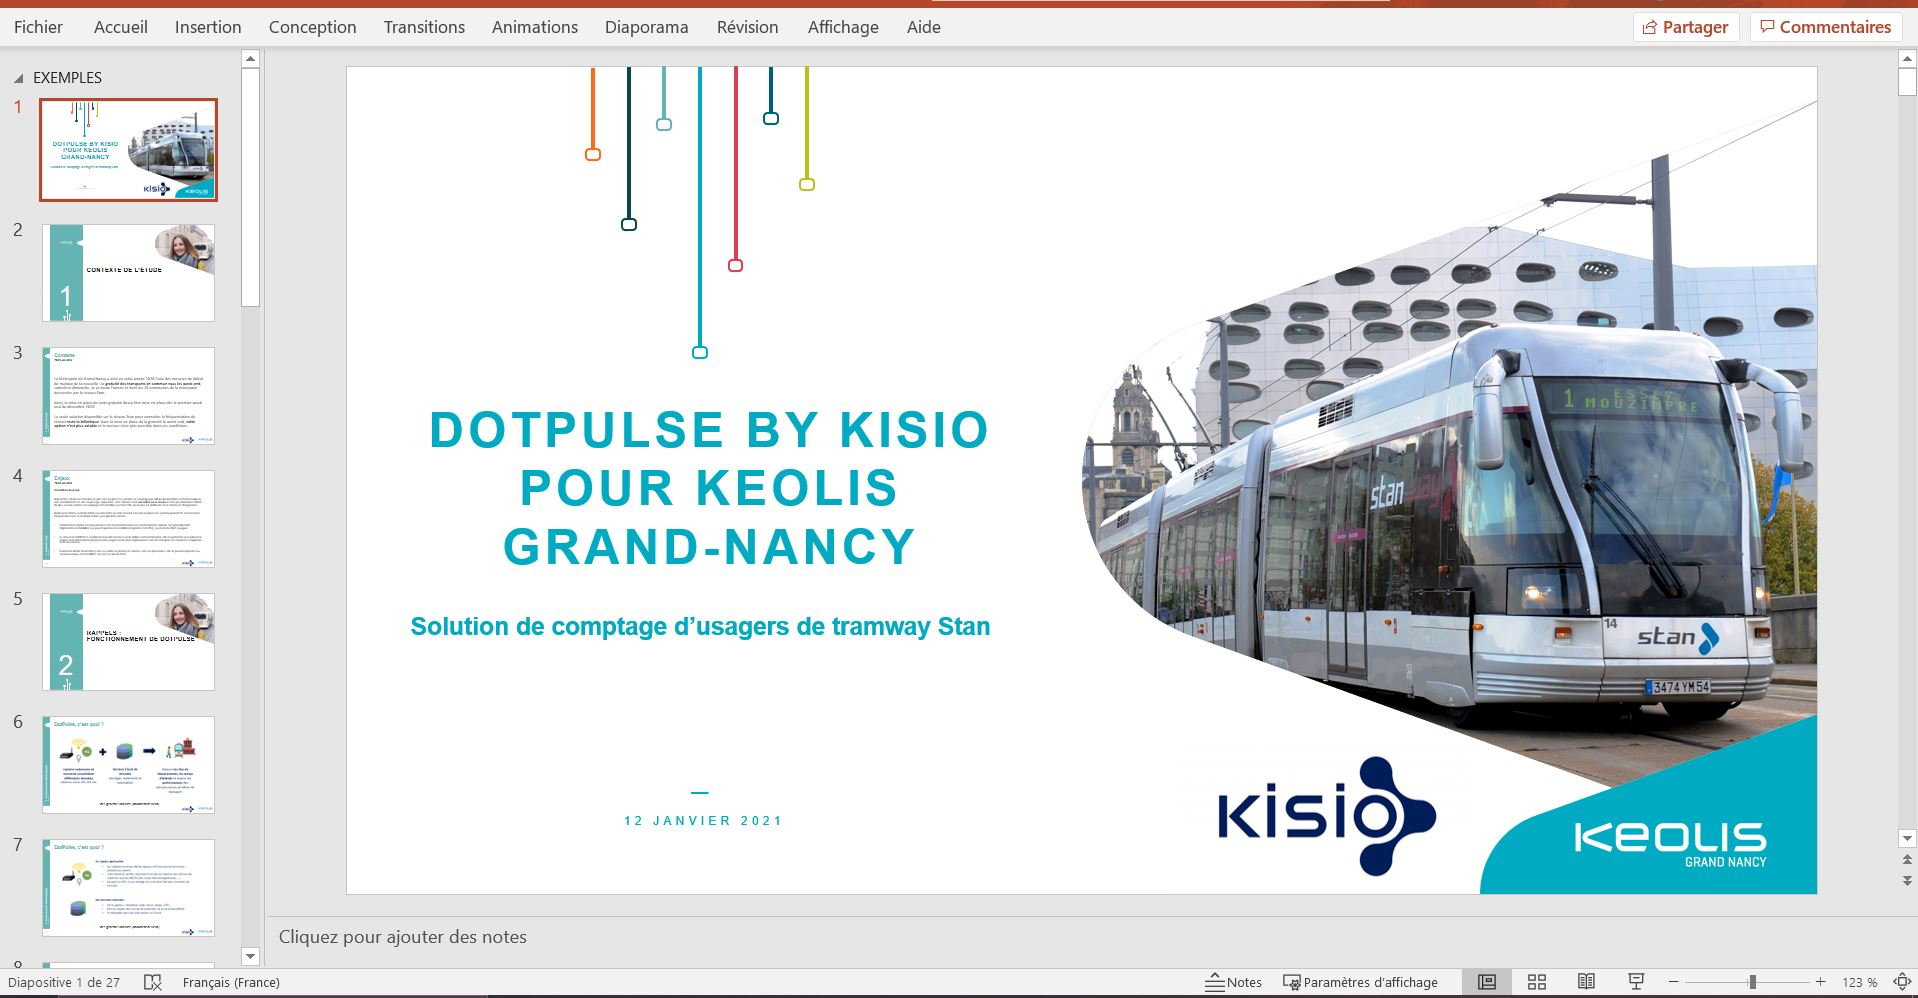
\includegraphics[scale = 0.4]{Images/DotPulse_presentation.JPG}
                \caption{Extrait de la présentation réalisée pour le projet DotPulse}
            \end{figure}
            
        \pagebreak
        \subsubsection{Gantt}

            \label{DotPulse_Gantt}
            \begin{figure}[!h]
                \centering
                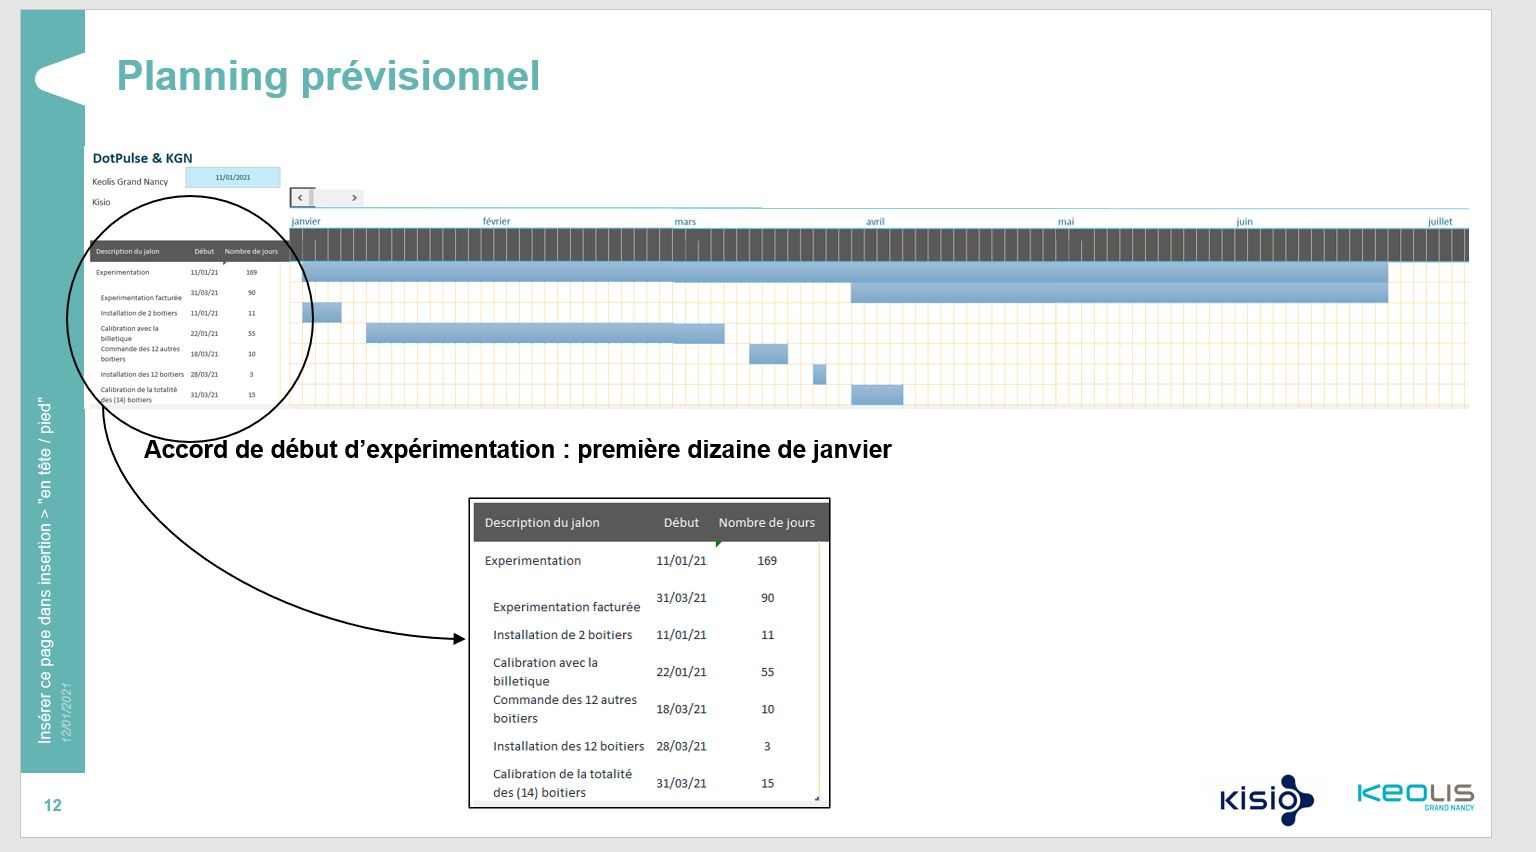
\includegraphics[scale = 0.5]{Images/DotPulse_Gant.JPG}
                \caption{Diagramme de Gantt réalisé pour le projet DotPulse}
            \end{figure}


    \pagebreak
    \subsection{Acorel}

        \subsubsection{La technologie}

            \label{Acorel_techno}
            \begin{figure}[!h]
                \centering
                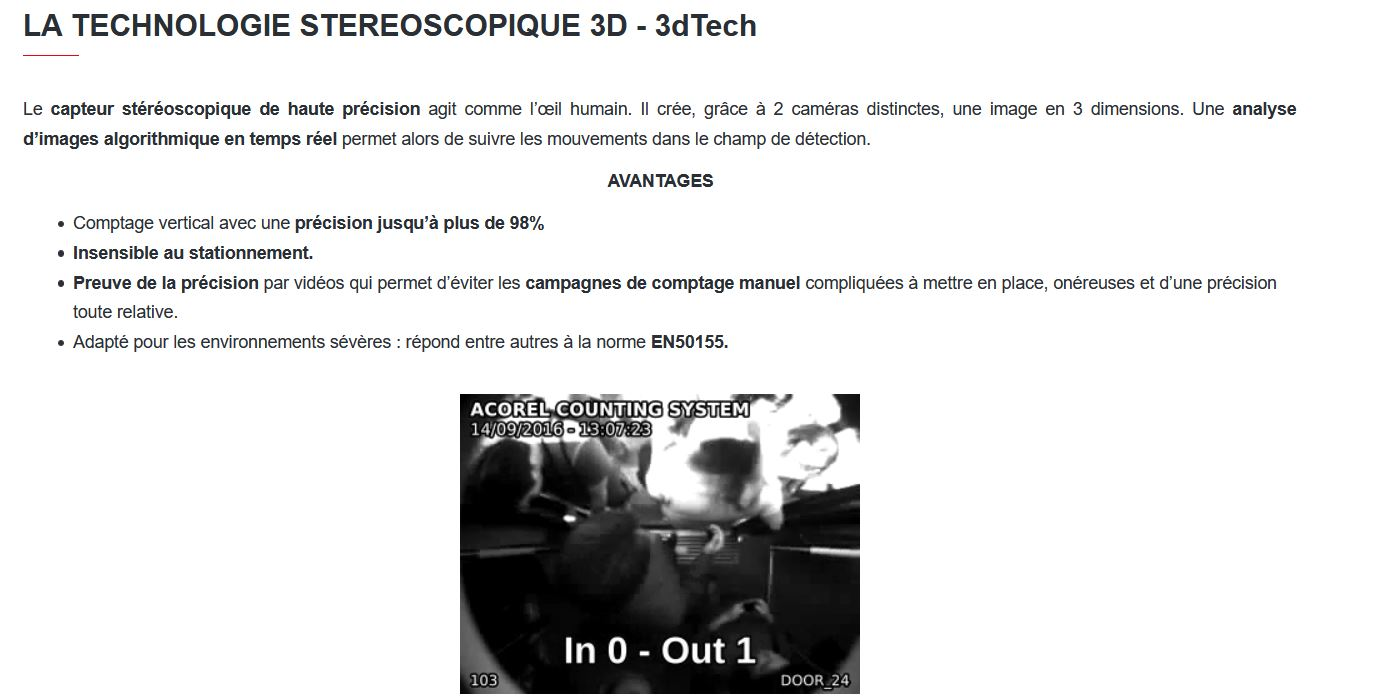
\includegraphics[scale = 0.5]{Images/Acorel_3d_tech.JPG}
                \caption{Présentation du principe de fonctionnement des cellules compteuses Acorel}
            \end{figure}

        \pagebreak
        \subsubsection{Etude}
            \label{Acorel_etudes}
            \begin{figure}[!h]
                \centering
                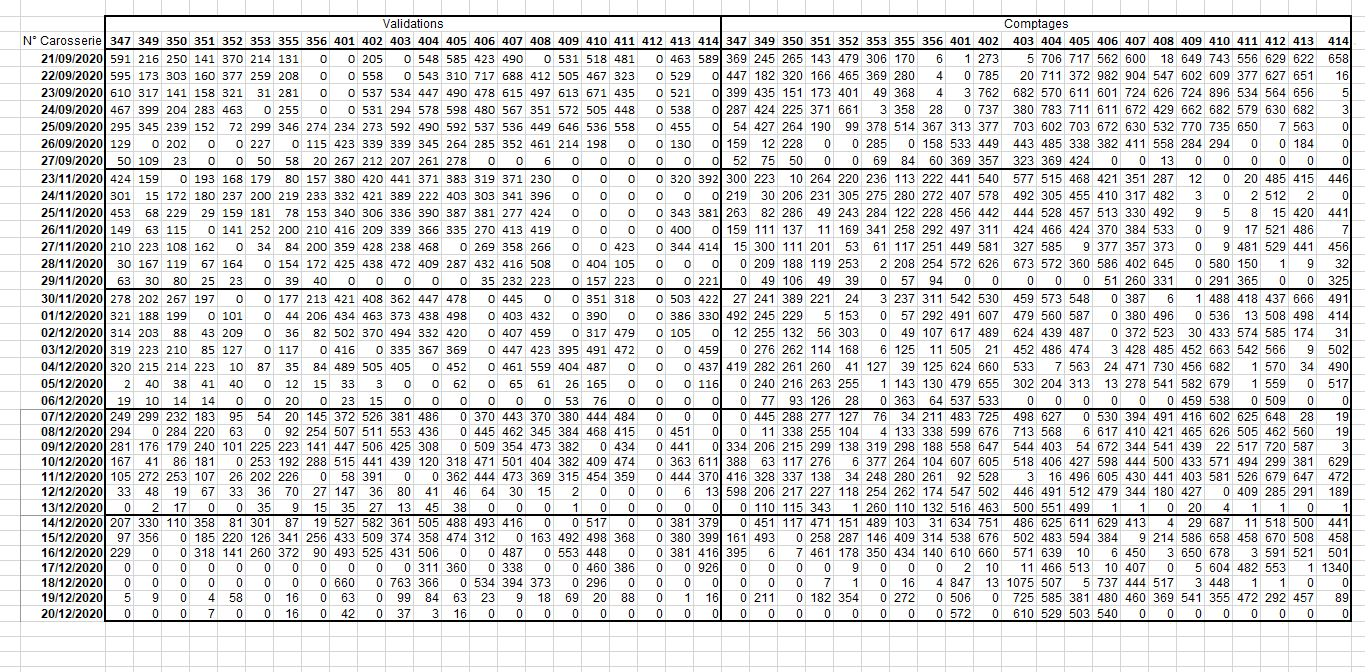
\includegraphics[scale = 0.5]{Images/Acorel_bilan.JPG}
                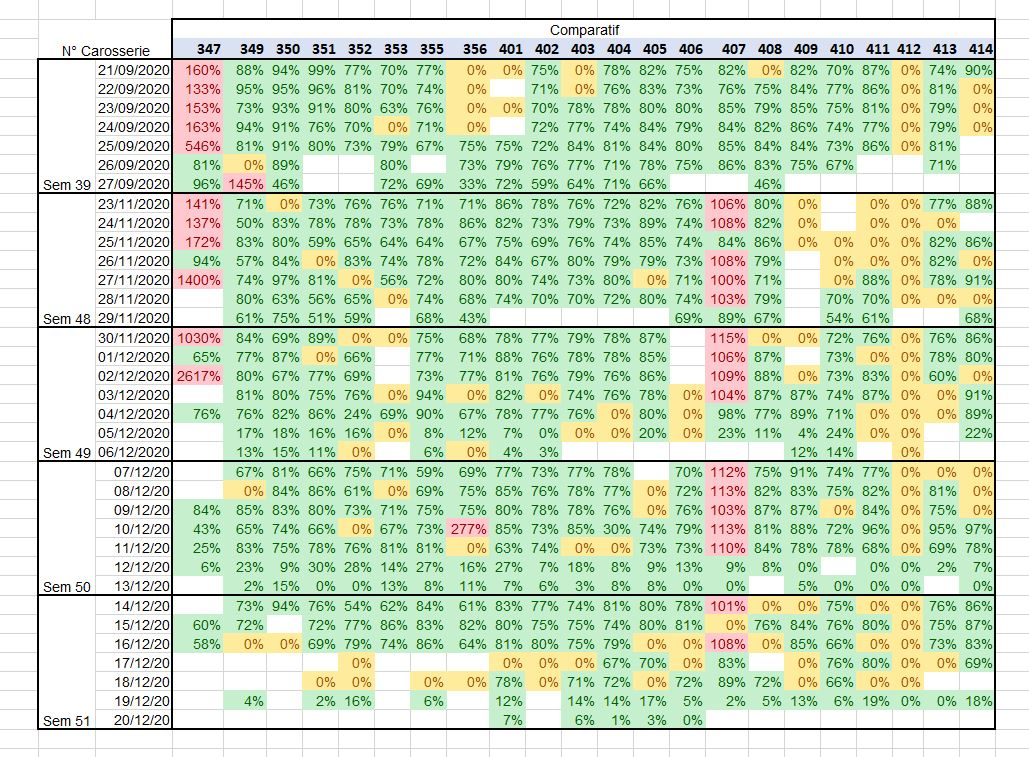
\includegraphics[scale = 0.7]{Images/Acorel_comparatif.JPG}
                \caption{Présentation du travail d'étude Acorel}
            \end{figure}

    \pagebreak
    \subsection{GLPI}
        \subsubsection{Interface}
            \label{Gpli_ex}
            \begin{figure}[!h]
                \centering
                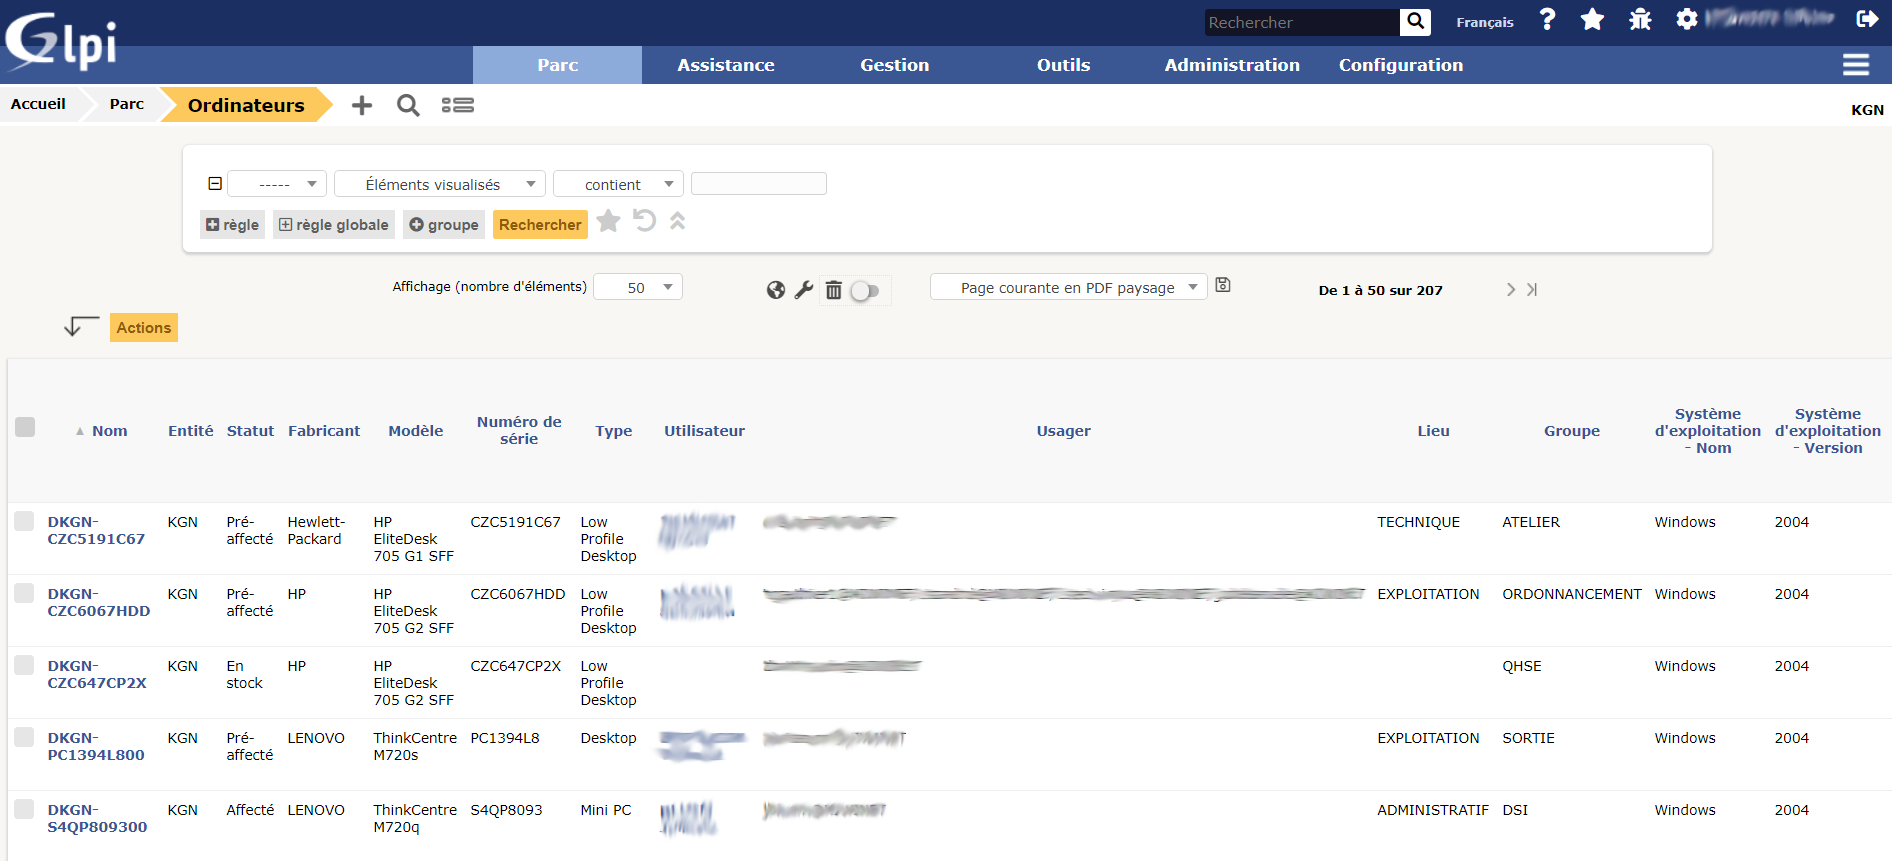
\includegraphics[scale = 0.32]{Images/GLPI.png}
                \caption{Exemple de l'interface GLPI}
            \end{figure} 
        \pagebreak
        \subsubsection{Version papier}
            \label{Gpli_papier}
            \begin{figure}[!h]
                \centering
                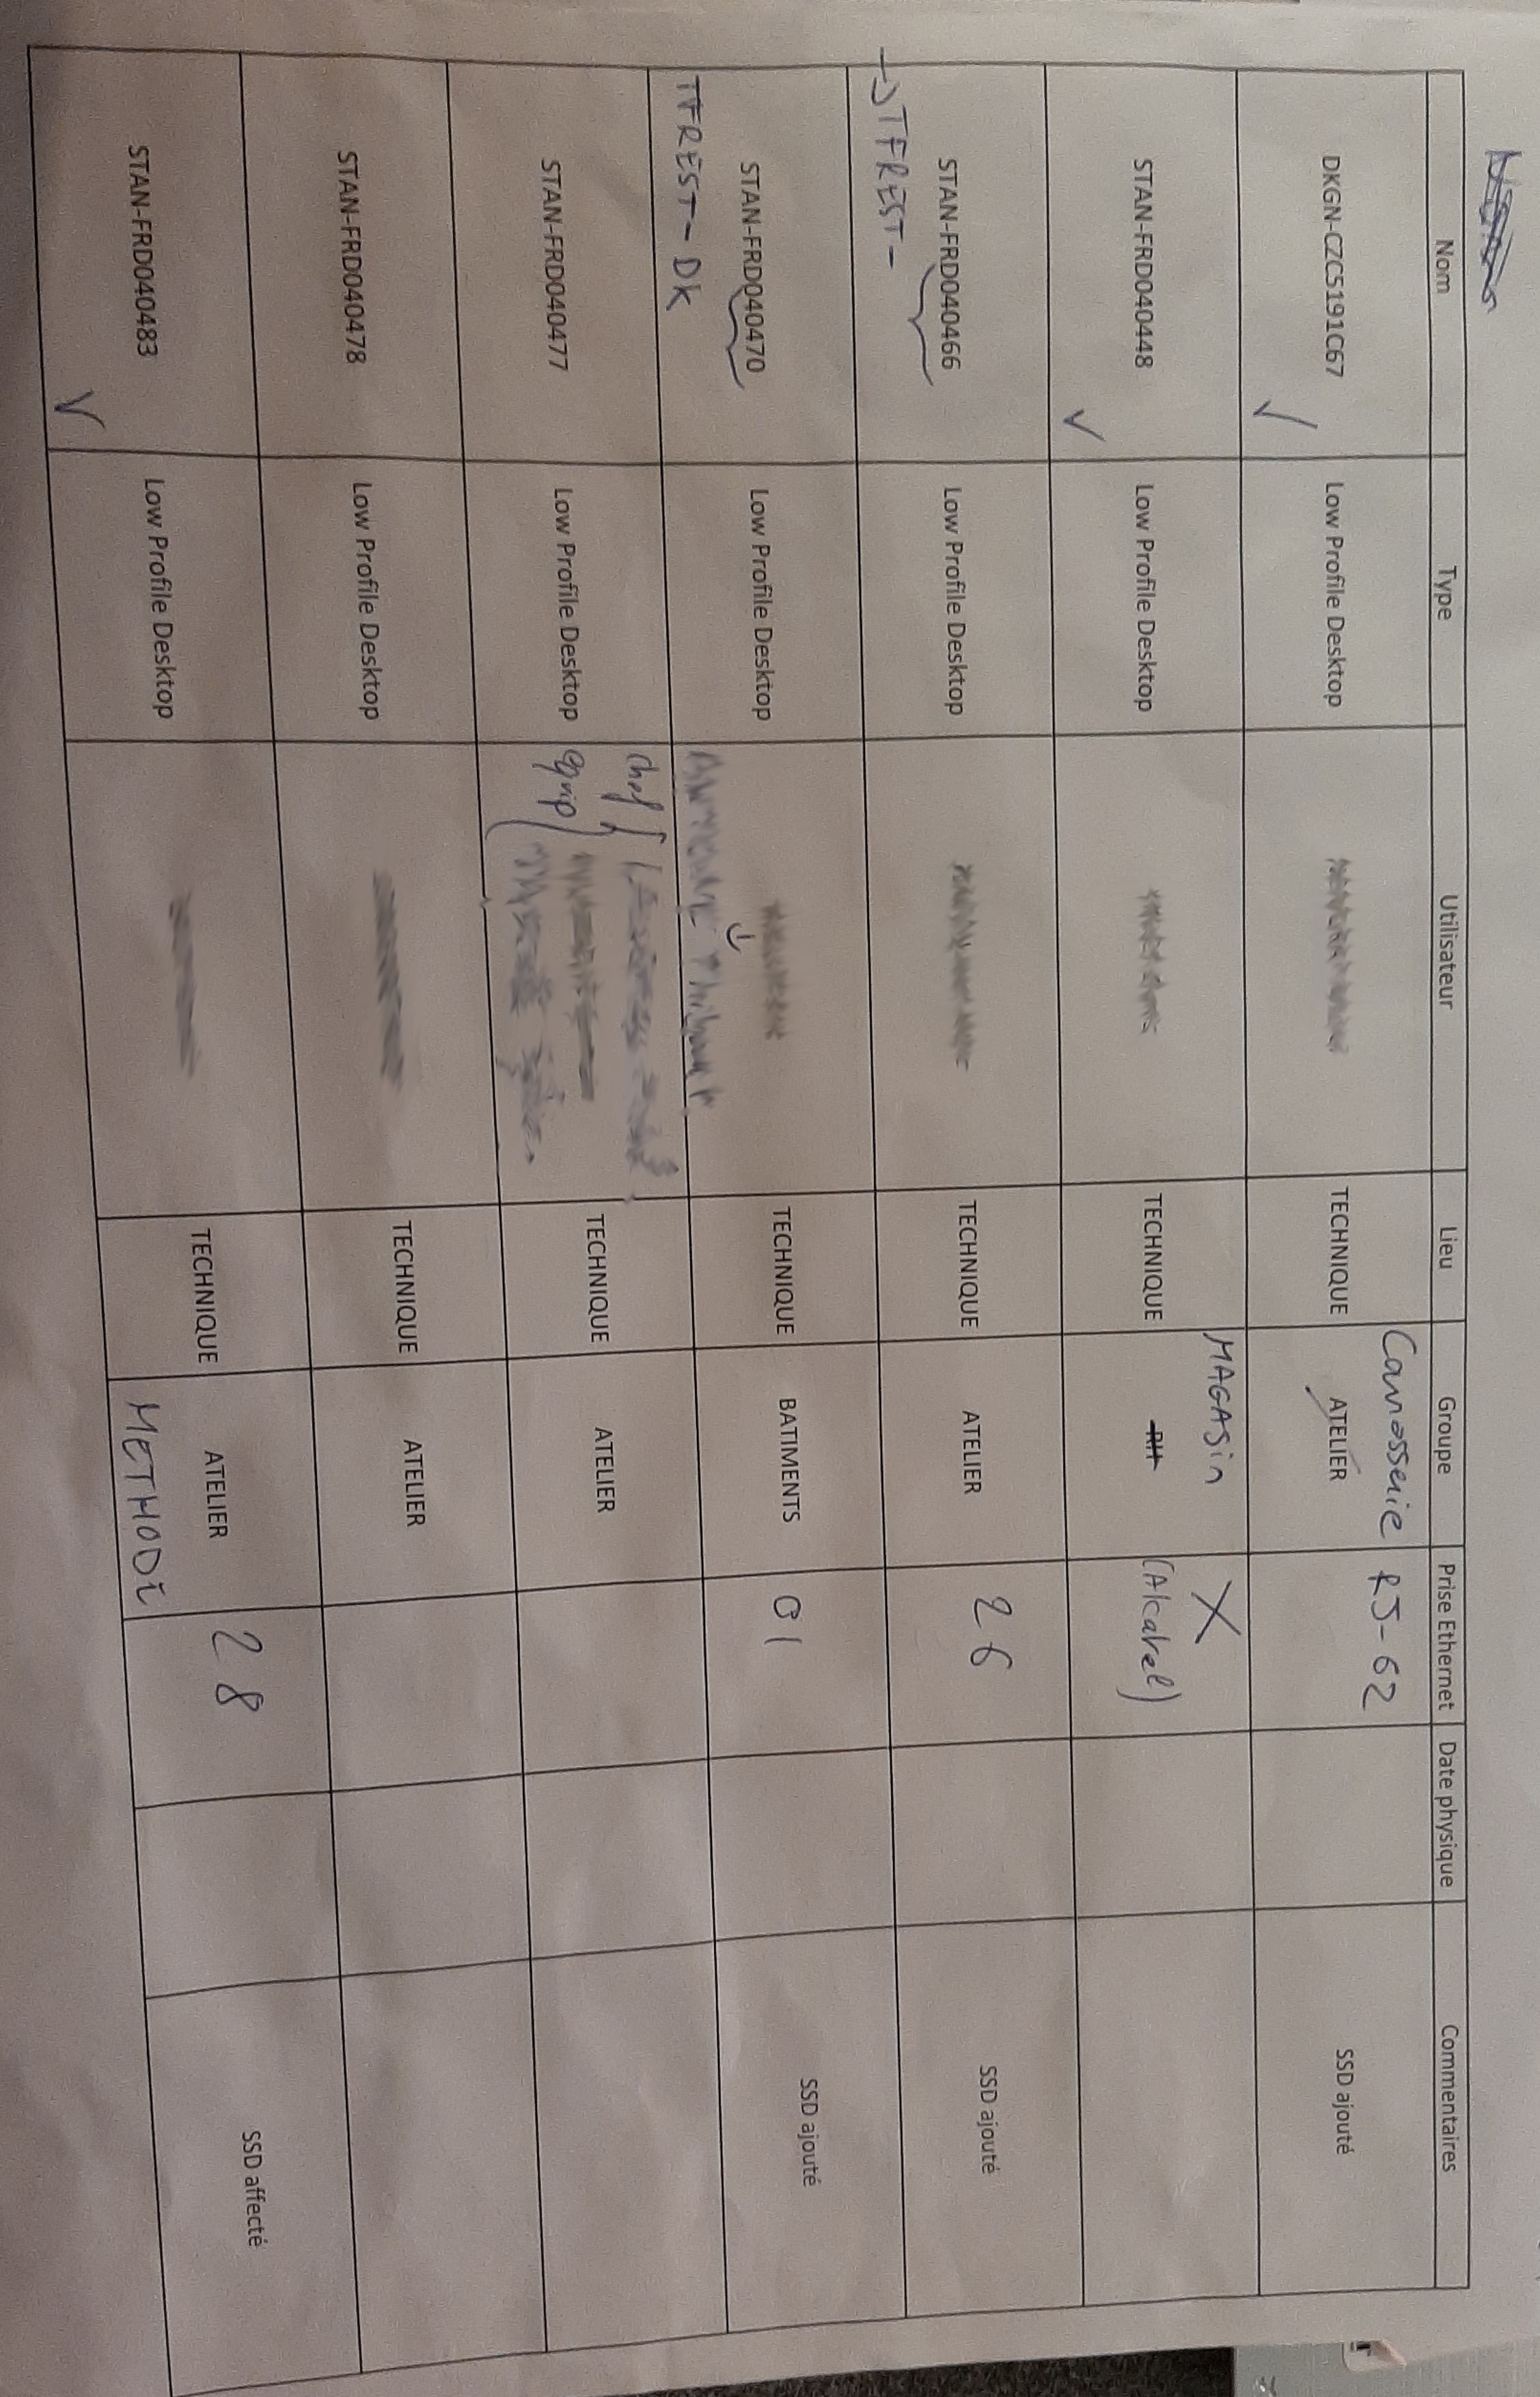
\includegraphics[angle = 90, scale = 0.17]{Images/Inventaire.jpg}\\
                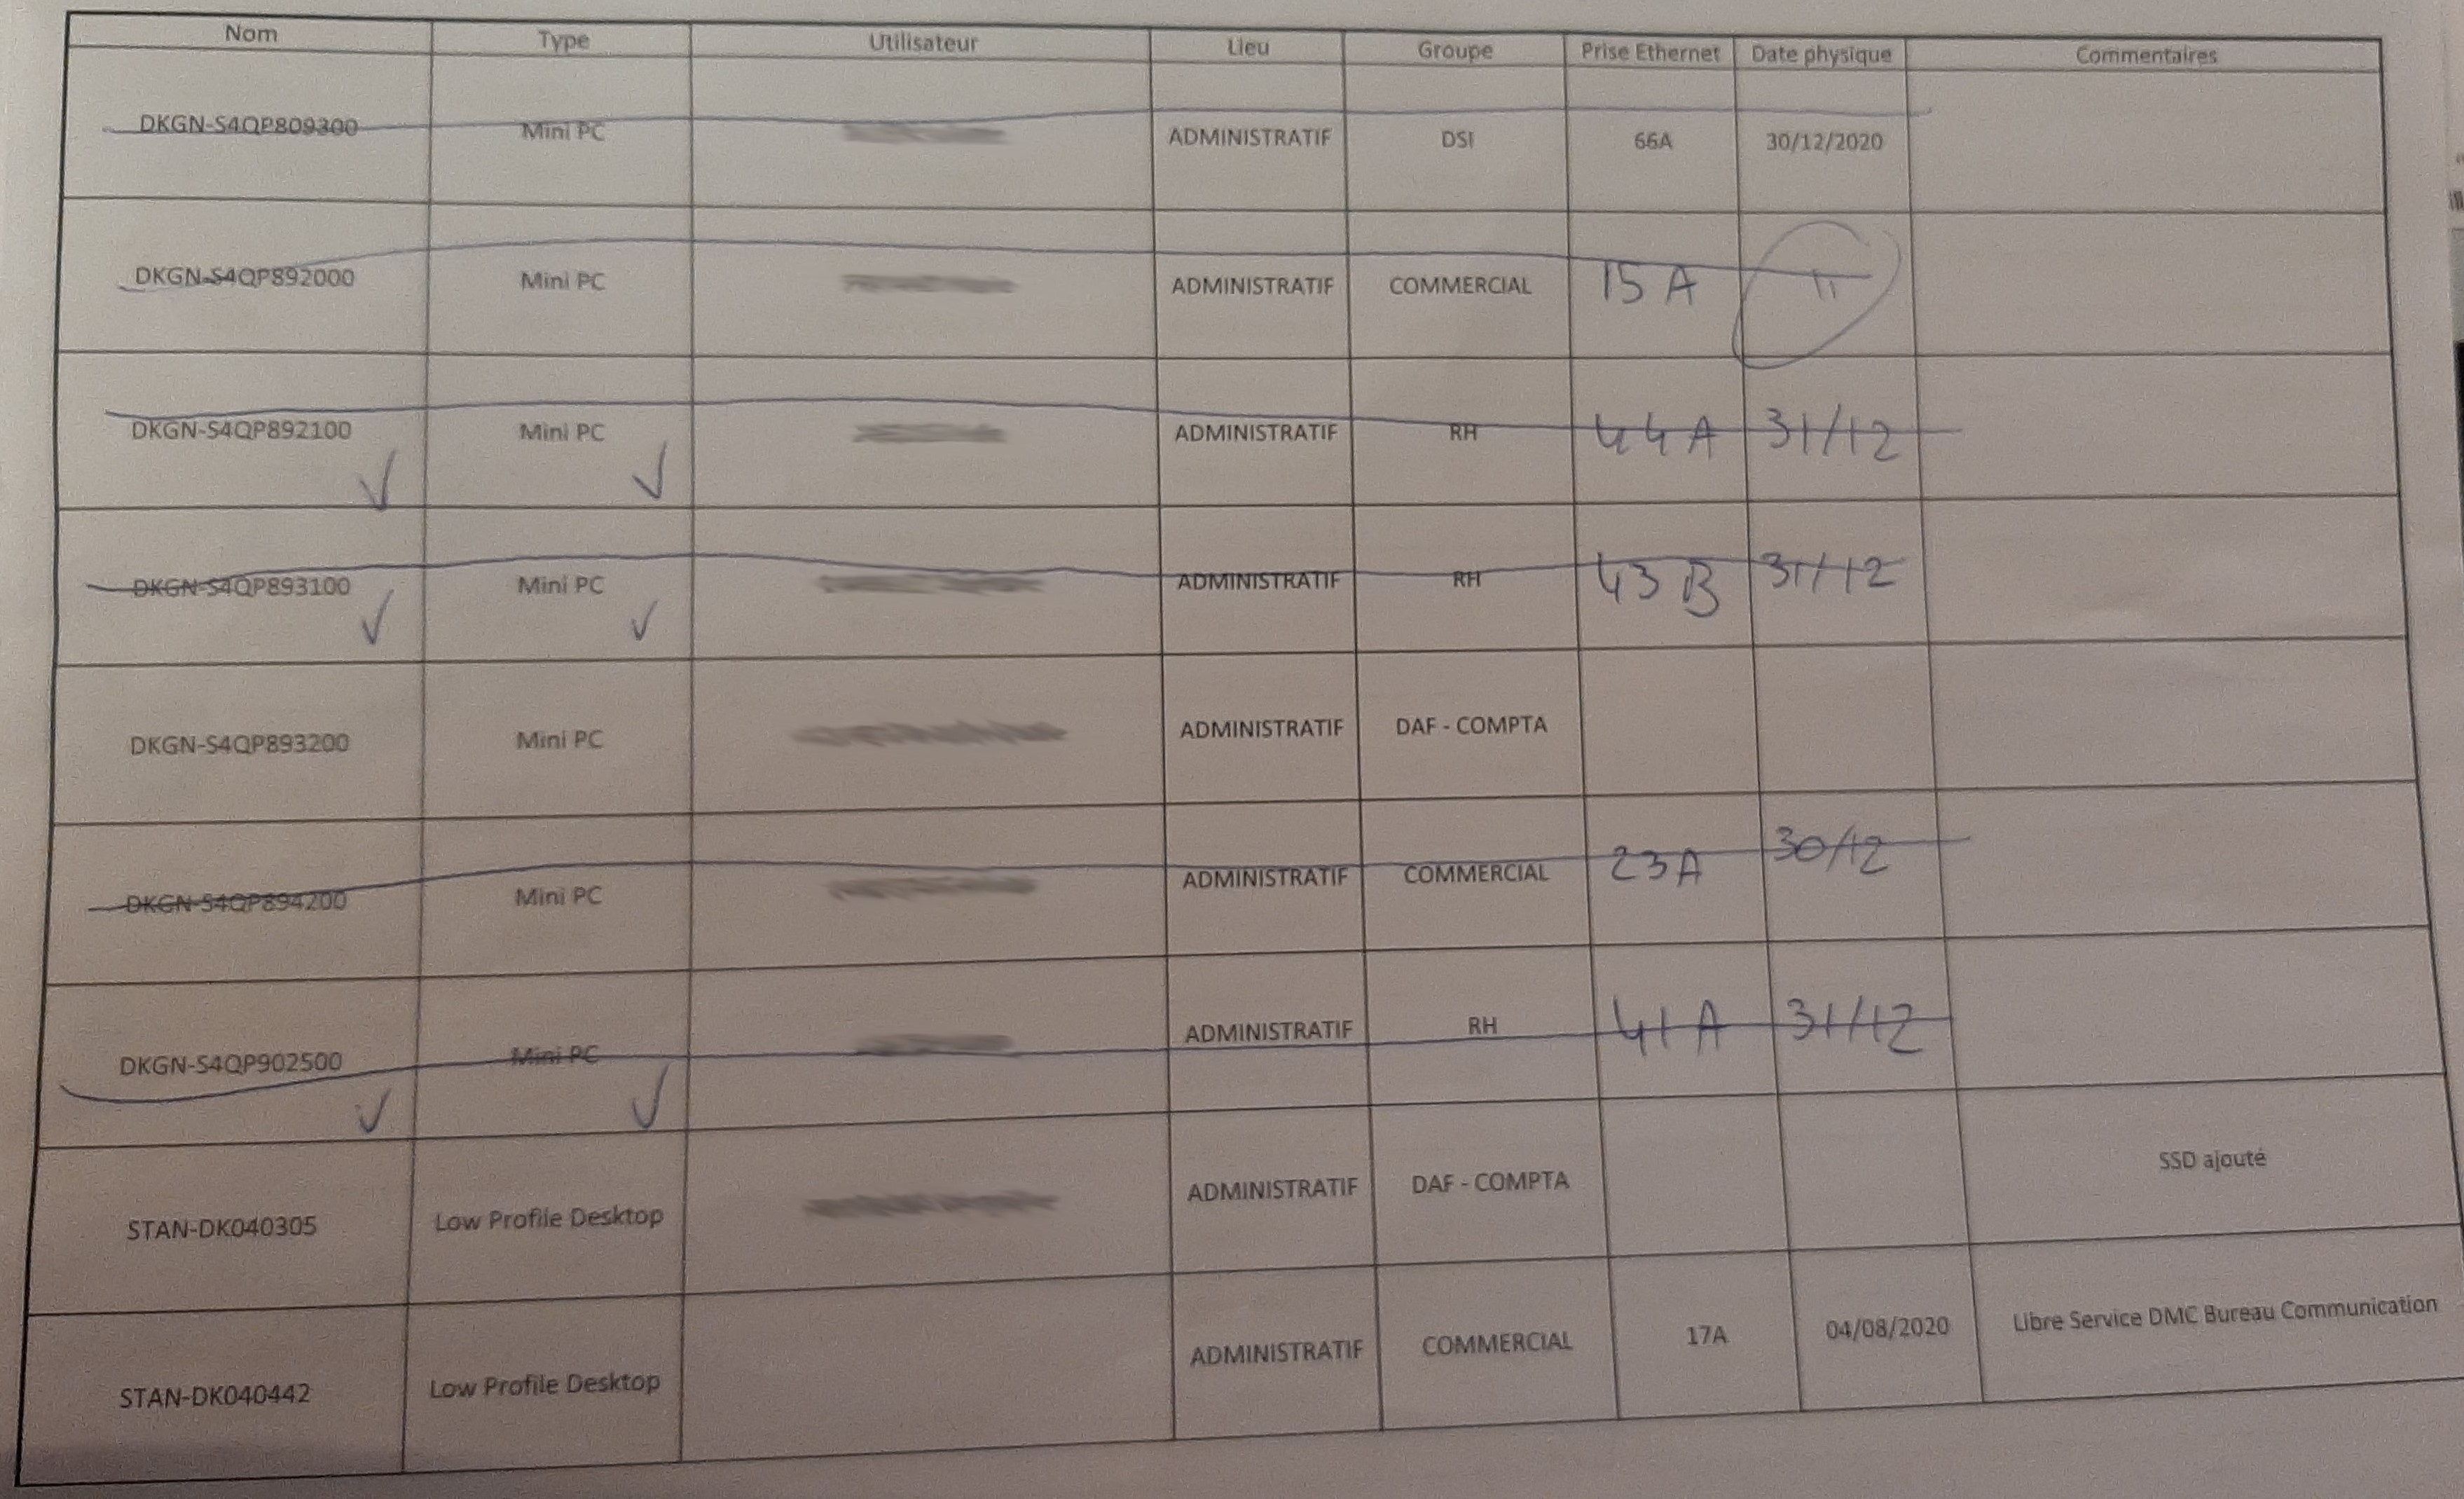
\includegraphics[scale = 0.127]{Images/InventaireRaye.jpg}
                \caption{Version papier avant de compléter GLPI}
            \end{figure}

\end{document}
